\chapter{Other exercises in motif discovery}
\section{Introduction}

The previous two chapters of this thesis were focused on
unsupervised methods for motif discovery, with an emphasis on
grammatical models.  Specifically, in Chapter 2 I demonstrated how
regular grammars can be used to model and design novel antimicrobial
peptides.  In Chapter 3, I addressed some of the weaknesses of
grammar--based motif discovery tools by developing a new approach
that is generic in the sense that it is applicable to many different
kinds of sequential data and is model agnostic.  In this chapter, I
continue this trend away from the core issues of grammar--based
motif discovery, to examine many closely related topics and
different approaches to motif discovery.

The first section of this chapter describes the development of an
efficient tool for matching regular grammars against large databases
of sequences.  The topic of the second section is the evolution of
amino acid scoring matrices over time.  As described in
Chapter~\ref{chapter:gemoda}, these matrices are the most common
metrics of protein similarity and are used widely by motif discovery
and sequence alignment programs.  The next section describes how
these scoring matrices and sequence alignment programs can be
co--opted for solving nontraditional bioinformatics problems such as
handwriting and voice recognition.  Finally, the last two sections
are devoted to exercises in motif discovery that do not use
grammatical methods, but instead rely heavily on classical machine
learning techniques and simple statistical analyses.

\section{Biogrep: a tool for matching regular expressions}\label{section:biogrep}


\subsection{Introduction}

As more genomes are sequenced and annotated, increasing numbers of
functional DNA and protein sequence motifs (or \emph{patterns}) are
being discovered. These motifs can be used to detect remote
homologies that are missed by sequence alignment tools such as
Blast~\cite{altschul1990basic} and FastA~\cite{pearson1998improved}.
Many databases such as Prosite~\cite{hofmann1999prosite},
PRINTS~\cite{attwood2003prints}, and
BLOCKS~\cite{henikoff1991automated} contain collections of
biologically significant patterns that are correlated with the
function of protein families and are expressed as regular grammars,
or equivalently, regular expressions (see
Section~\vref{section:regex}). For example, the Prosite the motif
\texttt{[AG]....GK[ST]} is indicative of ATP/GTP binding proteins.

Searching for such regular expressions can be an important part of
sequence annotation. There are a variety of tools available for
pattern--matching, the most common being the ``grep'' family of Unix
tools, including a number of very fast and sophisticated variants
such as agrep~\cite{wu1992agrep} and
NR--grep~\cite{navarro2001nrgrep}. Also, there are many excellent
bioinformatics--specific pattern--matching tools including
Patscan~\cite{dsouza1997searching}, tacg~\cite{mangalam2002tacg},
and fuzzpro~\cite{rice2000emboss}.  However, all of these tools are
optimized for searching for single patterns, that is,
one--at--a--time.

Biogrep is a pattern--matching tool designed to match large pattern sets
(100+ patterns) against large biosequence databases (100+ sequences) in a
\emph{parallel} fashion.  This makes biogrep well--suited to annotating sets of
sequences using biologically significant patterns.

\subsection{Implementation and results}
Biogrep is written in the C programming language using the GNU
regular expression~\cite{hargreaves1992regex} and POSIX threads
(pthreads)~\cite{mueller1993library} libraries.  The program reads
query patterns from either a plain text file, one--per--line, or
from a Teiresias--formated pattern
file~\cite{rigoutsos1998combinatorial} (see
Section~\vref{section:teiresias}). These patterns are treated as
POSIX extended regular expressions and are searched against a user
supplied file, which can be either a FastA--formatted biosequence
database or any text file.

Table~\vref{table:biogrepPerformance} shows a comparison of Biogrep
with a few common programs.  The grep family of pattern matching
tools are absent from the table because their run times are extremely
long.  This is because many of these tools cannot take sets of patterns
and have to be used on a per pattern basis.  The next best alternative
to Biogrep is a simple PERL script split between multiple
processors.

\begin{table}[!h]
    \centering
    \caption[Performance of Biogrep matching all the
        1333 patterns in Prosite.]{
        Performance of Biogrep matching all the
        1333 patterns in Prosite (release 17.01)
        against the 782370 protein sequences in
        Swiss--Prot/TrEMBL~\cite{bairoch2000swiss-prot}
        (release as of 8 July 2002).  Runs were
        carried out on an IBM p670 eserver
        running AIX 5L with 8 Power4 processors.
    }
    \label{table:biogrepPerformance}
    \vspace{2mm}
    \begin{tabular}{ccc}\hline\hline
        program & \# processors & execution time (s)  \\ \hline
        biogrep & 1 & 8683 \\
        biogrep & 2 & 4477 \\
        biogrep & 4 & 2266 \\
        biogrep & 6 & 1620 \\
        perl & 1 & 11780 \\
        perl & 6 & 1916 \\
        patscan & 1 & 28466 \\
    \hline\hline
    \end{tabular}
\end{table}

Biogrep has a number of user options, which are described in the
documentation that comes with the software.  Most importantly,
Biogrep can divide the pattern--matching task between a
user--specified number of processors using threads.  This
drastically reduces the user--time required to match large sets of
patterns (see Table~\vref{table:biogrepPerformance}). In addition,
Biogrep is distributed with detailed documentation, numerous
examples, and various helper--scripts for interfacing with other
pattern matching/discovery programs.  The Biogrep source code is
available at \url{http://web.mit.edu/bamel/biogrep.shtml}.

\clearpage
\section{The evolution of updated BLOSUM matrices and the Blocks database}

\subsection{Introduction}

As I discussed in Chapter~\ref{chapter:gemoda}, amino acid
substitution matrices are a very common way to measure the degree of
similarity between protein sequences (see for example
Section~\vref{section:gemoda-aa}). Indeed, the fidelity of amino
acid sequence alignment and motif discovery tools depends strongly
on the target frequencies implied by the underlying substitution
matrices. The BLOSUM series of matrices, constructed from the Blocks
5 database, is by far the most commonly used family of scoring
matrices. Since the derivation of these matrices, there have been
many advances in sequence alignment methods and significant growth
in protein sequence databases. However, the BLOSUM matrices have
never been recalculated to reflect these changes. Intuition suggests
that if the Blocks database has changed
--- by the growth or addition of blocks --- that matrices computed
after these changes may be different than the original BLOSUM
matrices.

Here we show that updated BLOSUM matrices computed from successive
releases of the Blocks database deviate from the original BLOSUM
matrices.  At constant re--clustering percentage, later releases of
the Blocks database give rise to matrices with decreasing relative
entropy, or information content.  We show that this decrease in
entropy is due to the addition of large, diverse families to the
Blocks database.  Using two separate tests, we demonstrate that
isentropic matrices derived from later Blocks releases are less
effective for the detection of remote homologs, and that these
differences are statistically significant.  Finally, we show that by
removing the top $1\%$ large, diverse blocks, the performance of the
matrices can largely be recovered.

This work is part of a manuscript that is currently under
consideration.  The manuscript was co--authored with Mark
Styczynski, Isidore Rigoutsos, and Gregory Stephanopoulos.
Throughout this section, the use of the pronoun ``we'' refers to
these authors.



\subsection{Motivation}

    Many different scoring matrices have been
    proposed in the literature, but the BLOSUM
    series~\citep{henikoff1992aminoacid} and PAM
    series~\citep{dayhoff1979amodel} of matrices are
    by far the most widely used.  For a review
    of the many different substitution matrices,
    the reader is referred to articles by~\citet{henikoff2000amino,henikoff1993performance}
    and~\citet{vogt1995assessment}.
    Despite the vast array of matrices available, a single matrix,
    BLOSUM62, has become a \emph{de facto} standard ---
    it is the default matrix for popular pairwise sequence alignment
    tools such as BLAST~\citep{altschul1990basic} and
    FastA~\citep{pearson1998improved} and multiple sequence
    alignment tools such as Clustal--W~\citep{thompson1994clustal}
    and t--coffee~\citep{notredame2000tcoffee}.

\begin{comment}
    The method used to create the Blocks database has its
    ancestor in the PAM matrices by Dayhoff~\citep{dayhoff1979amodel}.
    The PAM matrices are made by first collecting a
    database of proteins known to be closely related.
    From these, a common ancestral protein sequence is
    inferred and the mutations required to produce the
    descendant sequences are tabulated.  Because the set
    of descendant proteins is assumed to have diverged
    at the same time, the table of mutations can be
    interpreted as a rate of mutations.  By extrapolating
    this mutation rate matrix (by multiplying each matrix
    by itself an arbitrary number of times), amino acid substitution
    matrices for increasingly divergent sets of proteins
    can be constructed, e.g. PAM1, PAM120, and PAM250.
\end{comment}

    The BLOSUM series of matrices was constructed in 1992 from
    Blocks 5~\citep{henikoff1992aminoacid}: a database
    of protein blocks, or highly conserved protein regions, derived
    from families in the PROSITE database~\citep{hofmann1999prosite}.
    These blocks were used as a training set to derive a set of implied
    target frequencies that dictate the frequency with which an amino
    acid of one type should be aligned with an amino acid of another type.
    The various members of the BLOSUM matrix family --- BLOSUM100,
    BLOSUM62, BLOSUM50, etc. --- were made by clustering the sequences
    in each block at various thresholds, effectively down--weighting
    similar sequences to create matrices optimized for aligning more
    distant homologs.

    The Blocks database is itself used for homology
    searching~\citep{henikoff1994protein,pietrokovski1996searching}
    and other functions~\citep{rose1998consensus,ng2001predicting}.  As
    such, it is periodically updated, with ten major releases
    in the past ten years and some minor releases.
    Intuition suggests that these improvements in the Blocks
    database may make it a better training set for creating scoring
    matrices.  The goal of this manuscript is to show the effects of
    updates to Blocks on the matrices derived from the
    database.

    When the BLOSUM matrices were initially created and
    published, it was hypothesized that the use of more
    protein groups (and thus more blocks) in the matrices'
    creation would have little effect on the
    matrix~\citep{henikoff1992aminoacid}.  This was supported by the removal of
    specific blocks, or even half of the blocks, yielding approximately
    the same matrices.  However, in retrospect it is obvious that
    the known protein motifs in 1992 are a small fraction of those
    cataloged in today's databases.  Furthermore, it is plausible
    that motifs discovered ``early'' were inherently biased due to
    experimental methods and likely not representative of nature as
    a whole.  It is unclear whether new, more recent blocks would
    yield identical, similar, or significantly different matrices.

\begin{comment}
    Much attention has been given in the literature to the
    creation of optimized or specialized scoring
    matrices~\citep{sutormin2003batmas,muller2001nonsymmetric,lin2001amino}.
    Though the discovery of an incrementally better scoring matrix
    by updating the basis database may be of note, the discovery
    that worse matrices would result from such updates is just as
    important a conclusion, if not more so.  The discovery that a
    database's quality may be eroding, rather than improving, as more
    of the available biological data is incorporated leaves cause for a
    re--evaluation of the decisions made in maintaining the database.
    It is thus the aim of this work to perform a thorough evaluation
    of the effectiveness of possible BLOSUM matrices created with each
    major revision of the Blocks database.


    Here, we show that matrices derived from successive releases of
    the Blocks database are, in general, significantly poorer at a constant
    clustering percentage.  However, isentropic matrices --- that
    is, those with the same information content --- are only
    marginally poorer.
    \end{comment}

    In the following sections, we detail the construction of updated
    BLOSUM scoring matrices from successive releases of the Blocks
    database and describe the results of two sequence alignment tests
    used to evaluate the performance of these matrices.
\begin{comment}
    Somewhere else:

    On the whole, the matrices did not change drastically: most matrices
    were at least 65\% similar to the original BLOSUM62 matrix
    (recalculated appropriately).


    a comparison of updated BLOSUM matrices to the original
    BLOSUM matrix finds that about 25\% of the matrix entries
    are different.
\end{comment}
\subsection{Methods}

\subsubsection{Matrix construction}

All previous versions of Blocks databases were taken from the Blocks
ftp server, \url{ftp://ftp.ncbi.nih.gov/repository/blocks/unix/}.
BLOSUM matrices were constructed using a version of the BLOSUM
source code (available from the above FTP server) originally used to
prepare the BLOSUM family of matrices, but with some slight
modifications and bugfixes reported elsewhere~\citep{jensen2006all}.
These changes included fixing integer overflows in multiple
locations and fixing the weighting of substitutions between clusters
of sequences.  For each version of the Blocks database, a full scan
of all integer--valued reclustering percentages between $20$ and
$100$ was performed (Figure~\ref{fig:entropy}).  The matrix for each
Blocks release with relative entropy closest to the originally
reported BLOSUM62 matrix ($0.6979$) was selected as the
representative matrix for that release.

\begin{figure}[ptb]%figure1
\centerline{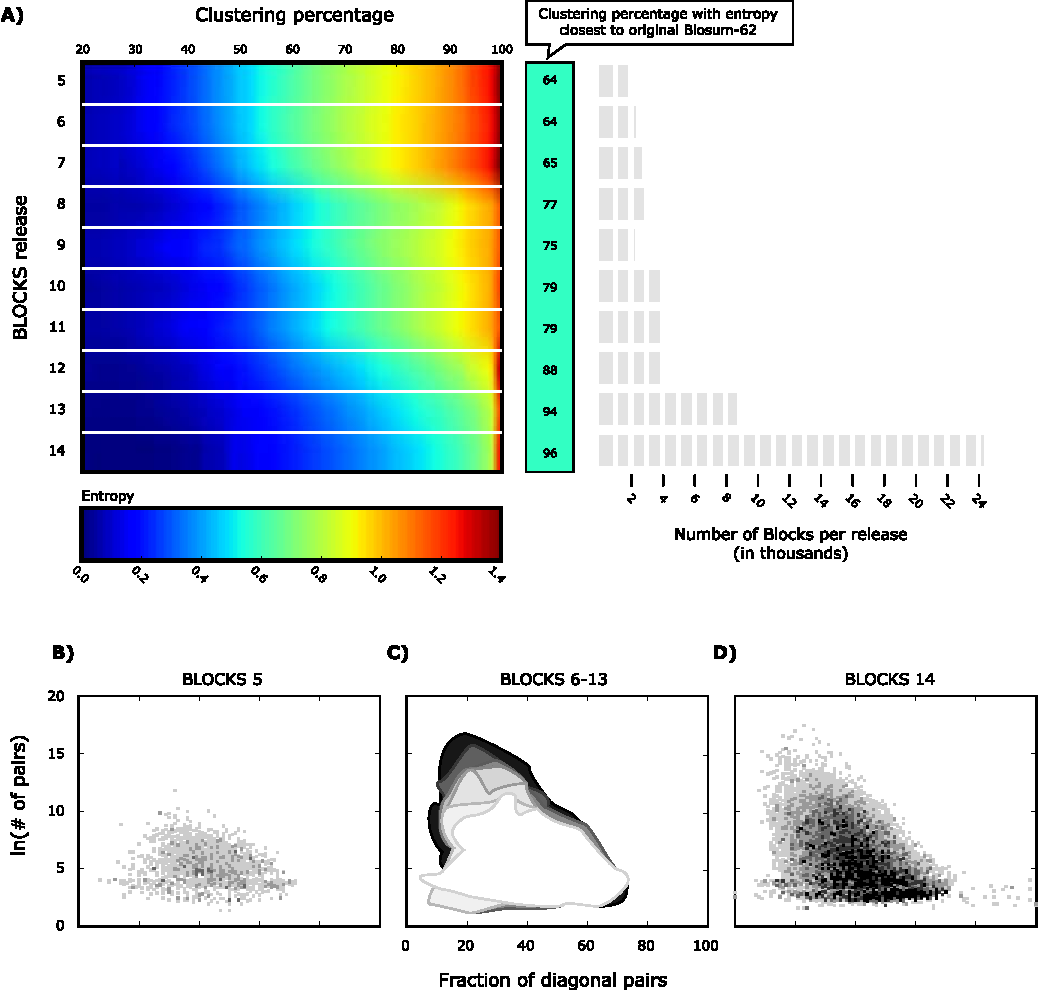
\includegraphics[width=\textwidth]{Body/Images-chap4/entropy-new.pdf}}
\caption[Characteristics of the BLOSUM matrices calculated from
successive releases of the Blocks database]{Characteristics of the
BLOSUM matrices calculated from successive releases of the Blocks
database.  Panel A) shows the entropy of the scoring matrices
computed from various Blocks releases as a function of the
clustering percentage used by the BLOSUM algorithm (see methods).
Blue colors indicate low entropies and red colors indicate high
entropies.  Oddly, at constant clustering percentage, matrix entropy
decreases with successive Blocks releases (see part B below).  The
middle part of panel A) shows the clustering percentage which
results in the matrix which has an entropy closest to the original
BLOSUM62 matrix.  The right--most panel shows the number of blocks
in each release of the Blocks database.  Panel B) of the figure
shows a scatter plot in which each block in the Blocks 5 database is
represented as a dot.  The location of the dot along the x-axis
represents the percent of the amino acid pairs contributed by that
block that lie along the matrix diagonal --- i.e. identical pairs
such as A--A, G--G, etc. The location of the dot along the y--axis
indicates the total number of amino acid pairs contributed by that
block.  (Note that the y--axis is in log units and that the matrix
was computed at 50\% clustering.)   Finally, panel D) shows the
scatter plot for Blocks 14. Notably, successive releases of the
Blocks database incorporated many large blocks comprising distantly
related sequences, as shown by the migration of the point clouds
towards the upper left quadrant. }\label{fig:entropy}
\end{figure}



\subsubsection{Sequence datasets}

Two different database searches were used to judge the ability of
each matrix to detect homologs: a search of SWISS--PROT
22~\citep{bairoch1992SWISS} using a set of queries previously
determined to reflect ``difficult'' searches that are able to
distinguish the abilities of different
matrices~\citep{henikoff1993performance}, and  a search of the
ASTRAL database~\citep{brenner2000astral} using each member as a
query.  These two different validation strategies have different
benefits: the former is historically relevant, as it was a method
used to initially demonstrate the superiority of BLOSUM62 to other
matrices~\citep{henikoff1992aminoacid,henikoff1993performance}. The
latter is more time--consuming, but it reflects current knowledge of
protein homology and allows for the determination of the statistical
significance of differences between matrices.

The first method we used for testing matrices was designed to
emulate the work by~\citet{henikoff1993performance}.  In that work,
the $257$ PROSITE 9.0~\citep{bairoch1991PROSITE} families that were
most challenging to detect were used as queries against SWISS--PROT
22 (numbering 25,044 sequences).  For each family, the list of all
members was used as true positives.

The second method we used for testing matrices was designed to
emulate the work by~\citet{price2005statistical}.  We used the
ASTRAL database~\citep{brenner2000astral} as the basis for our more
exhaustive experiments for detection of remote homologs.  ASTRAL is
created based on the SCOP database~\citep{murzin1995scop}, which
classifies proteins based on their function, structure, and sequence
into a hierarchical structure of classes, folds, superfamilies, and
families.  Sequences in the same superfamily can have low sequence
similarity, but are likely to have a common evolutionary origin
based on their structural and functional features.  Because these
classifications are made by human inspection, not via automated
sequence alignment procedures, it makes a perfect ``gold standard''
for remote homolog detection tests.

From the full set of ASTRAL genetic domain sequences, we chose the
sequence set from which $40\%$ identical sequences had been
eliminated. By using this subset, our search focuses on the
detection of remote homologs that are more challenging for
substitution matrices to discover and thus will differentiate the
abilities of the respective matrices to find distant relatives.  The
sequences were further filtered by
pseg~\citep{wootton1993statistics} for the removal of
low--complexity regions.  The unfiltered sequence set is available
on--line from the ASTRAL database at
\url{http://astral.berkeley.edu/scopseq-1.69/astral-scopdom-seqres-gd-sel-gs-bib-40-1.69.fa}.
This non--redundant set numbers 7,290 sequences.  Each sequence was
extracted from the database one at a time and used as a query for
the entire database.  Search results in the same superfamily as the
query were considered to be true positives.

\subsubsection{Search methods}

We chose the Smith--Waterman~\citep{smith1981identification} local
alignment algorithm for all searches against both databases for its
high sensitivity in detecting remote homologs.  In particular, we
used the ssearch implementation of the Smith--Waterman algorithm
by~\citet{pearson1990rapid,pearson1991searching}.

For our database searches, we used the ssearch default parameters
for unknown matrices, which are a -10 penalty for gap initiation and
a -2 penalty for gap extension.  We believe that these parameters
are reasonable settings; they represent an intermediate ground
between the values used in the initial BLOSUM paper (-8/-4) and
current commonly--used settings (for instance, the defaults for
BLOSUM62 in ssearch are -7/-1, while in BLAST they are -11/-1).
Moreover, previous work~\citep{gribskov1996useof} has shown that
while slight performance boosts can be found by optimization of gap
penalties, there is frequently a broad maximum of penalty values
with approximately equal efficacy.  In addition, a sampling of the
Kolmogorov--Smirnov statistic values returned by ssearch for
searches using our penalty values were well within the acceptable
range.  This indicates that the distribution of alignment scores is
the expected extreme--value distribution and that a significant
alteration of the gap penalties is most likely unnecessary.  That
is, our penalties are neither too forgiving nor too permissive.

Most importantly, the determination of completely optimized sets of
matrices and parameters is not the ultimate goal of this work.
Rather, the goal of this work is to analyze the BLOSUM matrices as
affected by the changing entries in the Blocks database.  In this
sense, the use of globally optimal parameters for each matrix is not
imperative; instead, the consistent use of some average, acceptable
parameter values for all matrices provides a level, controlled
environment for determining the relative raw ability of each matrix
to detect remote homologs.  So, though we feel we chose acceptable
parameters for our work, it is not of intrinsic importance to
determine the optimal parameters for each matrix.

It is worth noting that other works (particularly the early BLOSUM
works that the PROSITE--based testing method is based upon)
frequently used BLAST~\citep{altschul1990basic} instead of
Smith--Waterman to evaluate the quality of scoring matrices. In this
work, we chose Smith--Waterman because of its sensitivity and to
avoid any artifacts due to the heuristic shortcuts in BLAST.

\subsubsection{Evaluation of results}

For both sets of database searches, we used the same respective
methods for evaluating search results as in previous literature.  In
the PROSITE--based testing, we used head--to--head comparison of
effectiveness in finding family members.  For all PROSITE families
that were queried, the matrix that found the most true positives was
noted.  The relative effectiveness of any two matrices was then
found by subtracting the number of times that one matrix was more
effective from the number of times that the other was more
effective.  True positives were defined as described previously.
The search criterion used was the same as for the previous
work~\citep{henikoff1993performance}, as initially described
by~\citet{pearson1991searching}: if a true positive appeared before
$99.5\%$ of the true negative sequences, it was considered
``found''.

For ASTRAL--based testing, we used the Bayesian bootstrap method to
evaluate the statistical significance of the mean difference in
coverage between any two substitution
matrices~\citep{price2005statistical}. This method uses coverage vs.
errors per query as a means to evaluate the effectiveness of
different substitution matrices.  Coverage is defined simply as the
fraction of true positives found at a given errors per query
threshold. True positives were identified as described above.


\subsection{Results}

We began by first assembling the matrices that we would be using in
our experiments.  As stated in the Methods section, we used a
modified version of the original BLOSUM program that incorporated
multiple bugfixes. We created a matrix for each integer clustering
value between 20 and 100; the results can be seen in panel A of
Figure~\ref{fig:entropy}.

The center of panel A lists the reclustering percentage needed for
each Blocks release to produce a matrix with entropy closest to that
of the original BLOSUM62 matrix.  We used this set of isentropic
matrices for our sequence alignment tests.  A given matrix's
relative entropy reflects the required minimum length of homology in
order for it to be distinguished from
noise~\citep{altschul1991amino}.  Merely maintaining (in this case)
a reclustering percentage for a time--dependent family of matrices
would have little meaning, as changes in entropy could occur that
would obscure the effectiveness of the information encoded in the
matrix.  In this sense, it is only ``fair'' to compare matrices of
the same entropy.  Thus, we used matrices with the same relative
entropy of BLOSUM62, $0.6979$, which is approximately the value
previously shown to be most effective for database
searches~\citep{henikoff1992aminoacid}.  (Note that, due to the
bugfixes mentioned earlier, the BLOSUM matrix computed from Blocks 5
had its entropy analog at a reclustering percentage of $64$ rather
than $62$.)  We refer to matrices computed from the ``revised''
BLOSUM code as RBLOSUM, making the baseline matrix for that family
RBLOSUM64.

The right-hand side of panel A in Figure~\ref{fig:entropy} shows
that the number of blocks in each release increases in an almost
monotonic fashion, with the exception of release 9.  The general
trend is expected, as the PROSITE database that is used to create
the blocks would likely have more families of known homology added
in later releases.  The decrease in blocks in release 9 remains an
anomaly; we speculate that it may have been due to a one--time
change in parameters in the creation of the blocks, though we have
no way to verify this theory.

Inspecting the heatmap in panel A of Figure~\ref{fig:entropy}
reveals that, as expected, relative entropy increases with
increasing reclustering percentage in any given Blocks release.
However, at constant clustering percentage, matrices computed from
successive releases of the Blocks database show markedly decreased
relative entropy.  We hypothesized that this trend was due to
changes in the character of blocks in the database. Indeed, panels
B--D of Figure~\ref{fig:entropy} suggest that the presence of
extremely large, diverse blocks may have been the cause of this
phenomenon.  The scatter plots in panels B--D show point clouds
representing all the blocks in a given Blocks release (panel C shows
the outlines of these clouds).  Each block is represented as a
single point at a location that indicates the degree to which the
block contributes identical amino acid pairs (x--axis) and the total
number of amino acid pairs contributed by the block.  The three
panels show a trend towards the incorporation of blocks that have
many sequences that are only remotely homologous.  This trend is
manifested in the migration of the point clouds towards the upper
left quadrant of each of the three scatter plots.

These panels explain why the reclustering percentage needed to be
increased so much in order to create isentropic matrices. As large
blocks with more diverse sequences are added to the database,
something must be done to offset that diversity in order to obtain
an isentropic matrix. Since the highly diverse members of a family
(block) will not cluster together, they will have a significant
impact on the substitution counts that are used to derive the
matrices. In order to offset this impact and steer the entropy of
the matrix away from that of the background, it is necessary to
increase the re--clustering percentage used to compute the matrices.
In this way, blocks containing highly homologous sequences will have
greater influence on the substitution counts and steer the matrix
closer to the desired counts and information content.

Having assembled a set of isentropic matrices, we then used our two
tests --- the historical, PROSITE--based test and the statistically
rigorous, ASTRAL--based test --- to evaluate the effectiveness of
updated BLOSUM matrices. By using both of these tests rather than
just one, the comparison of updated substitution matrices is
grounded in the same metrics as would have been used when the
matrices were first published, while providing quantitative
statistical results.

We found that, with time, the character and quality of the entries
in the Blocks database has changed significantly.
Figure~\ref{fig:boxes} shows a slightly complex trend that warrants
some analysis.  The figure shows boxes whose vertical position
indicates their relative performance; the further a box is
vertically from the Blocks 5 box, the greater the difference in
performance between the isentropic matrices derived from those
releases (see caption).  In early updates of Blocks, the resulting
RBLOSUM matrices tended to hover around a certain performance.  This
is consistent with previous hypotheses~\citep{henikoff1992aminoacid}
that the BLOSUM matrix would not be altered by adding to or
subtracting from the Blocks database.  The variation could be
explained in part by integer rounding; since the desired scores are
rounded to the nearest whole number, it is possible that the
intended scores for a given matrix are not completely accurately
represented by a given BLOSUM matrix.  Another possibility is that
changing block quality causes these fluctuations; this possibility
is further analyzed below.  However, the particularly poor
performance of Blocks releases from 12 on, and that of release 9, is
inconsistent with the initial hypothesis that matrix performance
would remain approximately constant.


\begin{figure}[ptb]% figure 2
\centerline{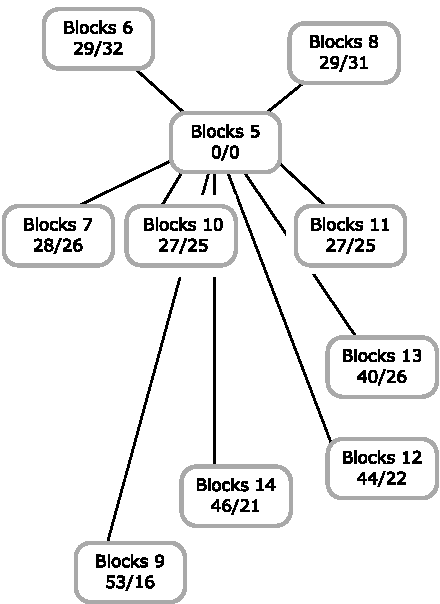
\includegraphics[width=0.50\textwidth]{Body/Images-chap4/henikoff-repo.pdf}}
\caption[The relative performance of updated BLOSUM matrices]{The
relative performance of updated BLOSUM matrices.  This figure is
designed to emulate Figure 4 from~\citet{henikoff1992aminoacid}.
All matrix performances are compared to the revised BLOSUM62
isentropic analogue derived from Blocks 5, RBLOSUM64.  Vertical
distance from Blocks 5 indicates relative performance, with matrices
above Blocks 5 performing better and those below it performing
worse.  Comparisons were based on the $257$ ``difficult'' queries
in~\citet{henikoff1993performance}, derived from PROSITE 9.0 keyed
to SWISS--PROT 22. Numbers in each box indicate the number of groups
for which RBLOSUM64 from Blocks 5 performed better than and worse
than isentropic matrices from other releases. Releases immediately
following Blocks 5 seem to cluster around the same level of
performance, while later releases (and release 9) have unusually bad
performance. }\label{fig:boxes}
\end{figure}

These results are largely consistent with our results from the
ASTRAL--based tests.  Figure~\ref{fig:bbs} is a representative
result for a set of Bayesian bootstrapping runs for the
ASTRAL--based test (in this case, for releases 5 and 14 of the
Blocks database).  The lighter, thinner lines track coverage as a
function of the allowed errors per query (EPQ) for individual
bootstrap runs, while the two thick lines represent the
full--database result.  Clearly, there is some overlap between the
two distributions, but a pairwise comparison of runs (as
demonstrated by the inset evaluated at 0.01 EPQ) shows a distinctly
non--zero difference between the two distributions.  The difference
in coverage at a variety of EPQ values can be used as a metric to
judge how consistently different the performances of any two
matrices are.

\begin{figure}[ptb]% figure 2
\centerline{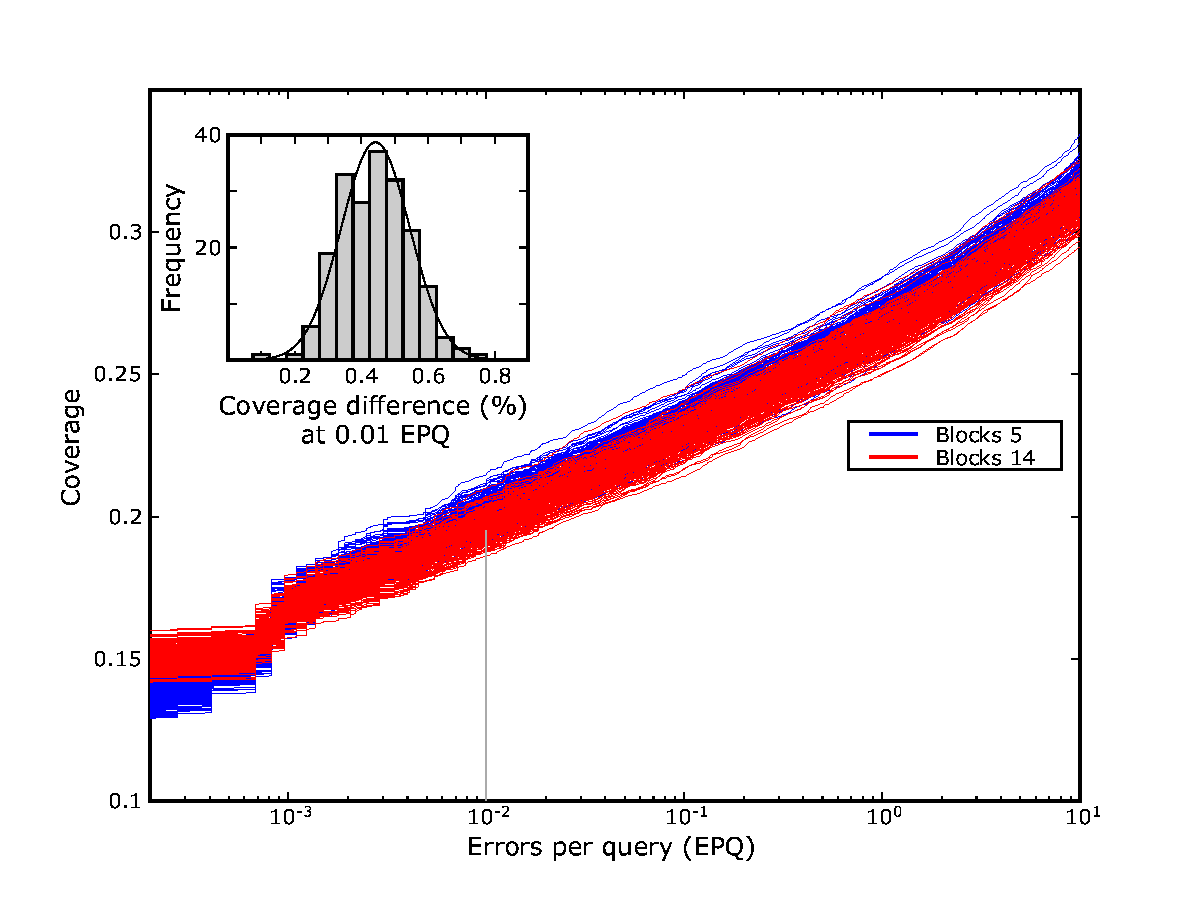
\includegraphics[width=\textwidth]{Body/Images-chap4/finalBbsWithInset.pdf}}
\caption[A complete set of Bayesian bootstrap replicates, with inset
histogram of coverage difference]{A complete set of Bayesian
bootstrap replicates, with inset histogram of coverage difference.
These data were created using the PSCE
software~\citep{price2005statistical}.
(See~\citet{price2005statistical} for a thorough explanation of
Bayesian bootstrapping).  Each thin, faintly colored line represents
one Bayesian bootstrap run.  The thick lines represent the total
dataset results.  In this case, the two distributions overlap
somewhat, but analysis of the data via the inset histogram of
coverage difference reveals that the difference in coverage clearly
follows a distribution with non--zero mean.  These distributions are
used to compute the confidence intervals shown in
Figure~\ref{fig:deltas}. }\label{fig:bbs}
\end{figure}

This metric is used in Figure~\ref{fig:deltas} to show the
performance of all updated matrices relative to the baseline
RBLOSUM64 matrix computed from Blocks 5.  These results correspond
quite well to the results in Figure~\ref{fig:bbs}.  That is,
releases 7, 8, 10, and 11 perform comparably to 5, release 6 is
slightly better, and release 12 is slightly worse, while releases 9,
13, and 14 perform substantively worse than release 5.  These latter
releases have statistically significant differences.  This agreement
suggests that the original test employed
by~\citet{henikoff1992aminoacid,henikoff1993performance} was rather
effective and efficient in that the results of the test would not
have changed much with access to today's larger databases.

\begin{figure}[ptb]% figure 2
\centerline{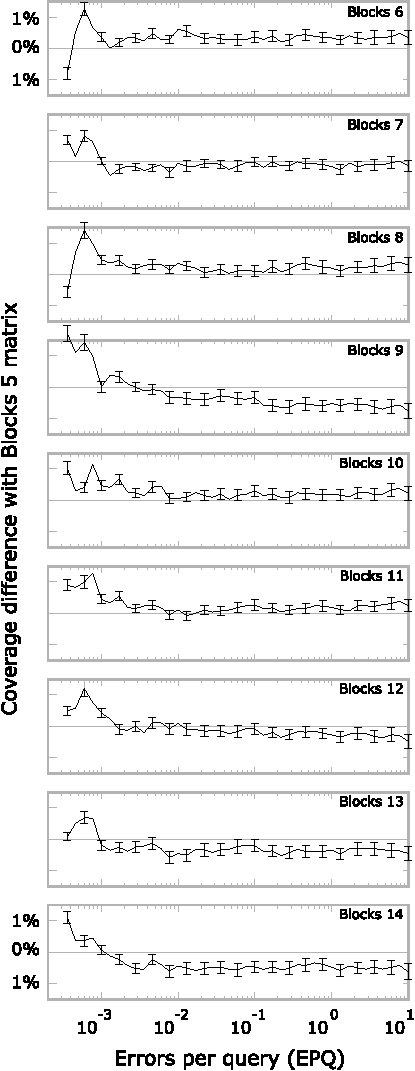
\includegraphics[width=0.40\textwidth]{Body/Images-chap4/fixedDeltas.pdf}}
\caption[Plots of the differences in performance of updated RBLOSUM
matrices]{Plots of the differences in performance of updated RBLOSUM
matrices. Each matrix is compared to the RBLOSUM64 matrix in 200
Bayesian bootstrap replicates to find the mean difference in
coverage, and the confidence interval for that coverage, at a
specific EPQ rate.  These differences are plotted as a function of
EPQ rate, with positive values meaning that a given matrix performs
better than RBLOSUM64 on the dataset. Error bars represent $95\%$
confidence intervals.  At data points where the error bars do not
intersect with the origin, the performance difference between the
matrices is statistically significant.  These results correlate well
with, and provide statistical analysis of, the results in
Figure~\ref{fig:boxes}. }\label{fig:deltas}
\end{figure}

\subsection{Discussion}
The reason for the poor performance of RBLOSUM matrices derived from
later releases of Blocks remains to be explained.
Figure~\ref{fig:entropy} suggests that the number of blocks and
shifting isentropic clustering percentage are not reasonable
explanations.  If these were so, one would expect to see either
gradually degrading performance (for database size) or significant
step changes in performance at releases 8, 12, and 13 (for
isentropic clustering percentage).  However, there is certainly not
a gradual degradation in performance, and there is no significant
change in performance at release 8.  In addition, any decrease in
performance at release 9 disappears for the next two releases.

We hypothesized that two phenomena --- the decreased entropy at
constant clustering in successive Blocks releases, and the poor
performances of these releases --- were both caused by the changing
character of blocks added in later releases.  Specifically, we
thought that the trends shown in panels B through D in
Figure~\ref{fig:entropy} might be responsible for these phenomena.

To test this hypothesis, we sorted the blocks in the Blocks 14
database by the number of off--diagonal (i.e., non--identity) amino
acid pairs contributed to the RBLOSUM matrix by each block. We then
removed the blocks that were the top $1\%$ of contributors to
off--diagonal pairs ($243$ blocks) and created an isentropic RBLOSUM
matrix from this ``cleaned'' database.  Notably, the reclustering
percentage required to create an isentropic matrix decreased from
$94$ to $84$ for the cleaned database.  The performance of this
matrix relative to RBLOSUM64 from Blocks 5 is shown in
Figure~\ref{fig:cleaned}. The cleaned version of the Blocks 14
database gives rise to an RBLOSUM matrix that is superior to any of
the other matrices we tested, including RBLOSUM64 from Blocks 5
(Figure~\ref{fig:cleaned}) and the original BLOSUM62 from Blocks 5
(data not shown).

\begin{figure}[ptb]% figure 2
\centerline{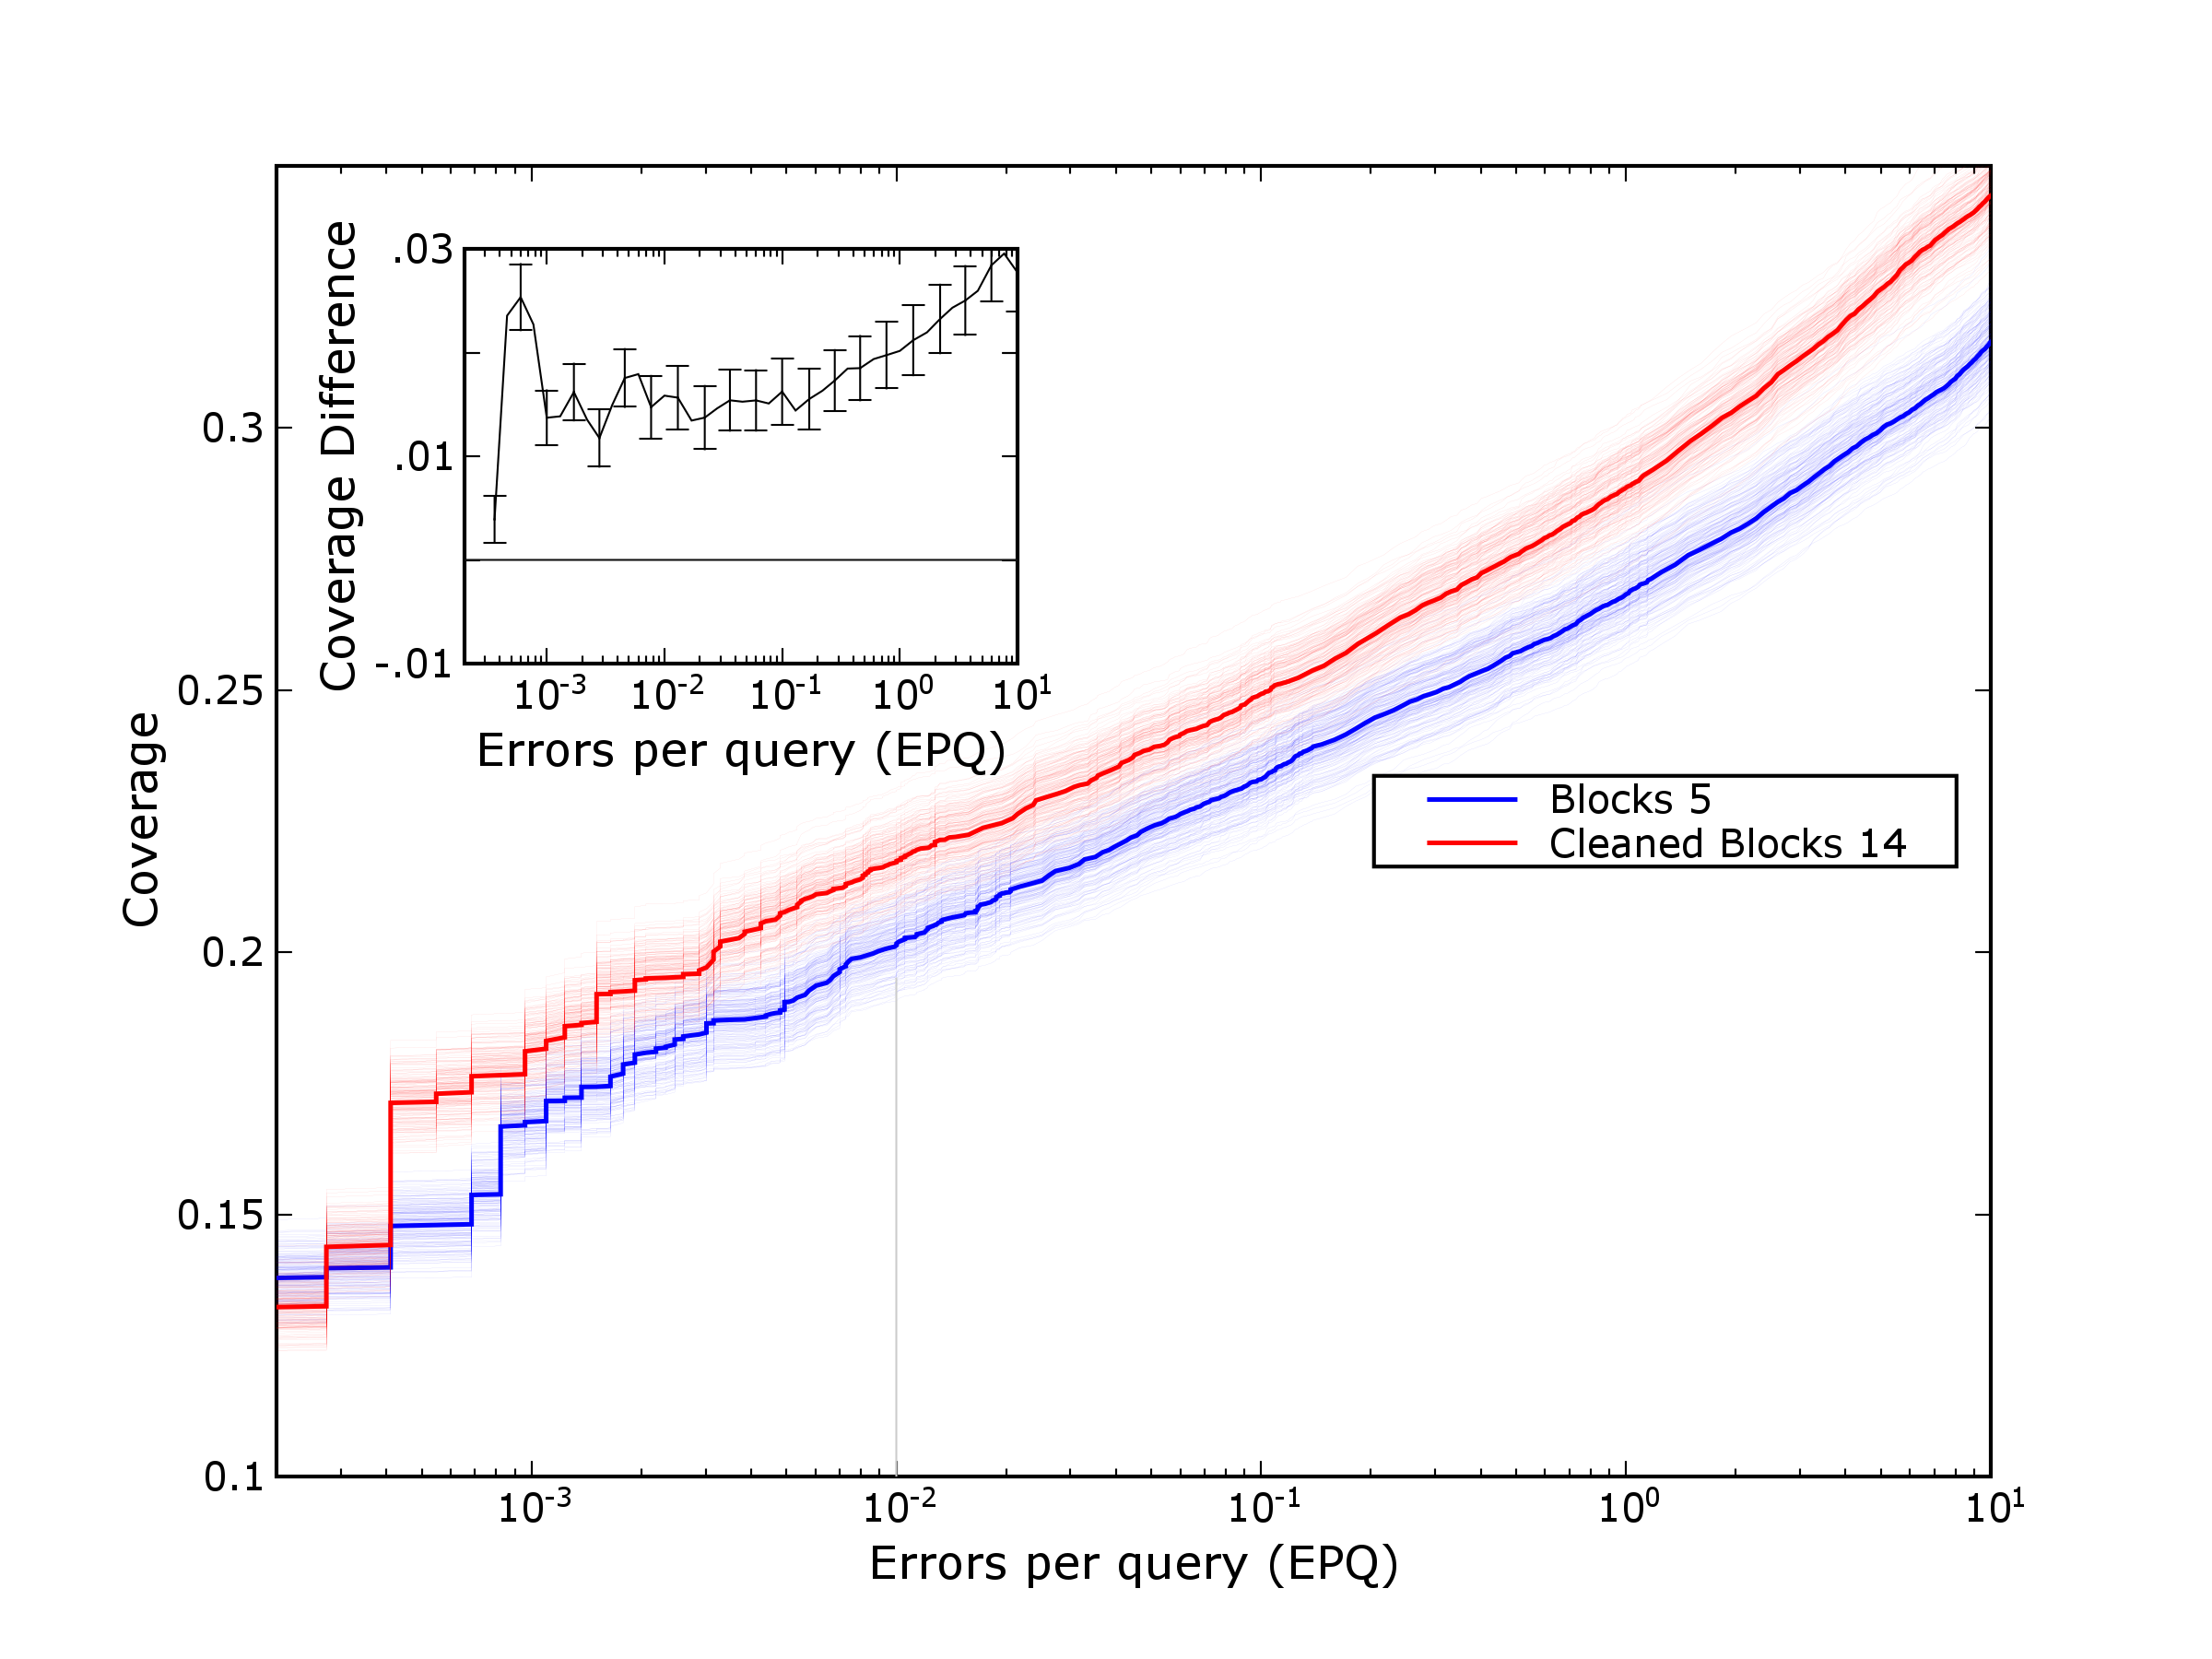
\includegraphics[width=\textwidth]{Body/Images-chap4/finalCleanedWithInset.png}}
\caption[Coverage of a cleaned RBLOSUM matrix compared to the
RBLOSUM64 matrix]{Coverage of a cleaned RBLOSUM matrix compared to
the RBLOSUM64 matrix.  Again, thin, faint lines represent individual
bootstrap runs, while the dark line represents the parent dataset.
These two distributions are quite distinct, with the cleaned RBLOSUM
matrix being significantly more effective than the RBLOSUM64 matrix
(and, transitively, all updated RBLOSUM matrices).  The inset shows
the coverage difference between the two matrices' coverage as a
function of errors per query.  Error bars represent $95\%$
confidence intervals.  Note the different scale from
Figure~\ref{fig:deltas} and the statistical significance at all EPQ
values since no error bar crosses the origin. }\label{fig:cleaned}
\end{figure}

The performance of the RBLOSUM matrix created from the ``cleaned''
Blocks 14 database supports our hypothesis that the addition of
large, diverse blocks has had an adverse effect on the performance
of updated RBLOSUM matrices. We believe that the decrease in
performance may be due to a change in the database that is used to
create the Blocks database~\citep{henikoff2005personal}.  Initially,
Blocks was based on the PROSITE database.  As of release 12 of
Blocks, blocks were formed from InterPro groups rather than PROSITE
groups. In release 12, only InterPro groups with cross--references
to PROSITE groups were used to create blocks.  In release 13, this
restriction was lifted, and it has remained lifted to the current
release of Blocks. We believe that this explains almost all of the
trends that we observe in the data.  When the Blocks database
partially shifted to being based on InterPro, performance first
decreased slightly with the addition of sequences that had not
previously been included.  When the shift was completed, performance
degraded significantly.  The only unexplainable anomaly is the
unusually poor performance of release 9 of Blocks; we believe that
can be attributed to the unusually small number of blocks in that
release.  Again, we speculate this may have been due to some
one--time change in parameters, but we have no way to prove or
disprove such a speculation.

In conclusion, we see that in some sense, the hypothesis
that~\citet{henikoff1992aminoacid} initially proposed was true: for
releases of the Blocks database based on PROSITE, despite some
slight variation, the performance of isentropic RBLOSUM matrices is
relatively constant over successive releases. However, since the
quality of the blocks added in recent releases has decreased, such
is not the case for the matrices derived from the current Blocks
database.  This suggests that, to the extent that there are ``bad''
blocks, there may also be ``good'' blocks, and sensible, judicious
selection of these blocks may be a reasonable approach for the
creation of amino acid substitution matrices.



\clearpage
\section{Bioinformatics and handwriting/speech recognition: unconventional applications of similarity search tools}
\subsection{Introduction}
    Bioinformatics has benefited immensely from tools and techniques imported
    from other disciplines.  Markov models used for gene--finding have
    their origin in information science, neural networks are imported
    from machine learning, and the countless clustering methods used
    for analyzing microarray data are from a wide variety of fields.

    Sequence alignment tools are no exception to this trend;
    however, within bioinformatics, they have reached
    new levels of speed and sophistication.  Tools,
    such as Blast~\cite{altschul1990basic,altschul1997gapped}
    and FastA~\cite{pearson1998improved}, are used routinely to search
    through a database for sequences (DNA or protein) that are
    similar to a query sequence.  Over the years, these tools have
    been optimized for speed by employing a number of heuristic
    shortcuts to the dynamic programming algorithms on which
    they are based.  Even searches in very large databases,
    such as Swiss--Prot/TrEMBL~\cite{bairoch2000swiss-prot} or
    GenBank~\cite{benson2000genbank}, take only a few seconds
    for queries of small to moderate size.  This is substantially
    faster than the time required for a rigorous Smith--Waterman
    search~\cite{waterman1984efficient}.  In light of the remarkably
    speed and accuracy that characterize these algorithms, it is
    intriguing to investigate other applications where similarity
    search tools might be of material importance.  In this work, I present two
    alternative applications of these fast sequence alignment tools
    outside the domain of bioinformatics: handwriting recognition and
    speech recognition.  All of the work described in this section
    is part of a publication appearing in the proceedings of the fourth
    Singapore--MIT Alliance Programme on Molecular Engineering of Biological and Chemical
    Systems, which was co--authored with Gregory Stephanopoulos.
    Throughout this section, the use of the pronoun ``we'' refers to
    these authors.

    The dynamic handwriting recognition problem is to recognize
    handwriting from a touch tablet as found on personal
    digital assistants (PDAs), for example Palm Pilots, or tablet
    PCs~\cite{tappert1990thestate}.  These writing tablets sample
    the position of a pen as a function of time to produce a series of
    ($x,y$) points that are used by handwriting recognition algorithms to
    determine which character was written.  An excellent review of the
    most common algorithms is available from Plamodon and Srihari, 2000.
    These include feature analysis, curve matching, Markov models, and
    elastic matching, the last of which is based on dynamic programming
    and is related to both Blast and FastA.

    To apply similarity search concepts to the handwriting recognition
    problem, we represented the path of a PDA pen as a protein
    sequence by translating the ($x,y$) points into a string of
    amino acids.  Using the protein representation of handwriting
    samples, we were able to classify unknown samples with FastA.
    This is analogous to the problem of protein annotation using
    similarity searching: given a protein (a written character)
    of unknown function, we annotated the protein by searching for
    similar sequences (characters with similar ($x,y$) paths).

    We applied the same sequence alignment approach to speech
    recognition.  Automated phone services, security checkpoints,
    and computer dictation software employ some form of speech
    recognition.  Common speech recognition methods include feature
    recognition, neural networks, hidden Markov models, dynamic
    programming~\cite{ney2000progress} and a variety of other statistical
    and signal processing algorithms.  A good review of these techniques
    and more is available from Juang \& Furui, 2000.  For this problem,
    we represented digital speech recordings as sequences of amino
    acids, and used a database of annotated recordings to classify
    unknown recordings.

    In the following section, we describe the data sets used for the
    handwriting recognition and speech recognition problems.  Then,
    we detail how these data were represented using strings of amino
    acids and how we used FastA to annotate unknown samples in four
    handwriting and speech recognition experiments.  We compare our
    results to more traditional methods of handwriting and speech
    recognition and, finally, we discuss ways of improving upon the
    results and extending sequence alignment to other classification
    problems.

        \begin{figure}[ptb]
                \centering
                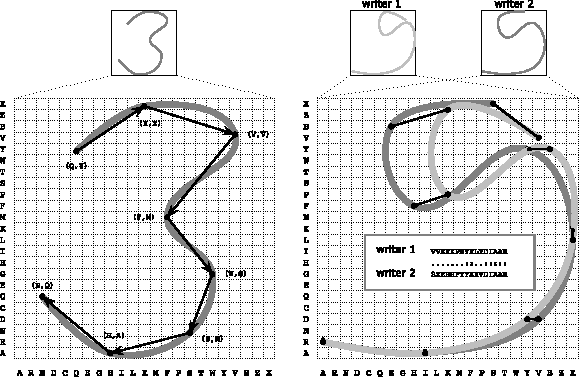
\includegraphics[width=\textwidth]{Body/Images-chap4/digits.pdf}
            \caption[Projection of a digit written with
                    a PDA stylus into protein space]{Projection of a digit written with
                    a PDA stylus into protein space.
                    Concatenating the set of
                    points gives a protein sequence
                    representative of the digit.
                    In this case, the sequence is
                    \texttt{QYKXVVFMWGSNHANQ}.%
                    An alignment of nines from two
                    different writers.  The boxes at
                    the top show the input from each
                    writer and the large grid show the
                    superposition of the two handwritten
                    digits.  The FastA alignment between
                    the protein representations of the
                    two digits is shown in the center.
                Two visualizations of the handwriting
                recognition problem.  In both cases the
                $x$ and $y$ axes are divided into 23 parts
                corresponding to the columns and rows in
                an amino acid scoring matrix.  The eight
                sampled points from the digit are cast from
                $x,y$ space into protein space by assigning
                amino acid coordinates to each point.
            }\label{fig:pda}\label{fig:pdaAlign}
        \end{figure}

        \begin{table*}[ptb]
            \centering
            \caption[Misclassification results for the handwriting and
                speech recognition problems]{Results for the handwriting and
                speech recognition problems described
                in the text.  For each experiment,
                the misclassification is the percent of
                sequences in the unknown set for which the
                digit or letter was not predicted correctly.}
            \subtable[
                Handwriting recognition results.
            ]{
\begin{tabular}{ccc}\hline\hline
Experiment & Classification & \parbox{4.8cm}{\centering \vspace{1mm}Classification in\\
Alimoglu \& Alpaydin, 1996\vspace{1mm}}  \\ \hline
1 & 97.34\%  & 97.80\% \\
2 & 99.64\% & n/a \\
%3 & 0.46\% & n/a \\
\hline\hline
\end{tabular}
} \subtable[Speech
                recognition results.
                The second column shows the
                misclassification using the clustering of
                all /ee/ sounding letters as described in the
                text.  ]{ 
\begin{tabular}{cccc}\hline\hline
Experiment & Classification & \parbox{2.5cm}{\vspace{1mm}Classification\\ with clustering\vspace{1mm}} & \parbox{4.5cm}{\centering \vspace{1mm}Classification in\\
Dietterich \& Bakiri, 1995\vspace{1mm}} \\ \hline
1 & 93.84\% & 98.91\%  & 96.73\% \\
2 & 92.61\% & 98.61\% &  n/a \\
%3 & 5.11\% & 0.71\% & n/a \\
\hline\hline
\end{tabular}
 }
            \label{table:results2}\label{table:results1}
        \end{table*}


        \begin{table*}[ptb]
        \centering
        \caption[Handwriting alignment scoring matrix]{The scoring matrix used for the handwriting
            and speech recognition FastA alignments.
            Each entry of the scoring matrix, $s_{ij}$, is given by $s_{ij}= 10-(|i-j|)$.
            That is, matching amino acids are given 10 ``points'', amino acids
            that are one off are given 9 points, and so on.  This matrix was used
            in place of the default scoring matrix,  Blosum50~\cite{henikoff1992aminoacid},  for FastA.
            The scoring matrix was found heuristically.  Also, a few experiments indicated that the
            alignments are relatively insensitive to permutations about the form of $s_{ij}$ given above.

        } \label{table:matrix}
        
\tiny
 \begin{tabular}{c@{\hspace{2mm}}c@{\hspace{2mm}}c@{\hspace{2mm}}c@{\hspace{2mm}}c@{\hspace{2mm}}c@{\hspace{2mm}}c@{\hspace{2mm}}c@{\hspace{2mm}}c@{\hspace{2mm}}c@{\hspace{2mm}}c@{\hspace{2mm}}c@{\hspace{2mm}}c@{\hspace{2mm}}c@{\hspace{2mm}}c@{\hspace{2mm}}c@{\hspace{2mm}}c@{\hspace{2mm}}c@{\hspace{2mm}}c@{\hspace{2mm}}c@{\hspace{2mm}}c@{\hspace{2mm}}c@{\hspace{2mm}}c@{\hspace{2mm}}c@{\hspace{2mm}}c}\hline\hline
 & A & R & N & D & C & Q & E & G & H & I & L & K & M & F & P & S & T & W & Y & V & B & Z & X\\ 
A & 10 & 9 & 8 & 7 & 6 & 5 & 4 & 3 & 2 & 1 & 0 & -1 & -2 & -3 & -4 & -5 & -6 & -7 & -8 & -9 & -10 & -11 & -12\\ 
R & 9 & 10 & 9 & 8 & 7 & 6 & 5 & 4 & 3 & 2 & 1 & 0 & -1 & -2 & -3 & -4 & -5 & -6 & -7 & -8 & -9 & -10 & -11\\ 
N & 8 & 9 & 10 & 9 & 8 & 7 & 6 & 5 & 4 & 3 & 2 & 1 & 0 & -1 & -2 & -3 & -4 & -5 & -6 & -7 & -8 & -9 & -10\\ 
D & 7 & 8 & 9 & 10 & 9 & 8 & 7 & 6 & 5 & 4 & 3 & 2 & 1 & 0 & -1 & -2 & -3 & -4 & -5 & -6 & -7 & -8 & -9\\ 
C & 6 & 7 & 8 & 9 & 10 & 9 & 8 & 7 & 6 & 5 & 4 & 3 & 2 & 1 & 0 & -1 & -2 & -3 & -4 & -5 & -6 & -7 & -8\\ 
Q & 5 & 6 & 7 & 8 & 9 & 10 & 9 & 8 & 7 & 6 & 5 & 4 & 3 & 2 & 1 & 0 & -1 & -2 & -3 & -4 & -5 & -6 & -7\\ 
E & 4 & 5 & 6 & 7 & 8 & 9 & 10 & 9 & 8 & 7 & 6 & 5 & 4 & 3 & 2 & 1 & 0 & -1 & -2 & -3 & -4 & -5 & -6\\ 
G & 3 & 4 & 5 & 6 & 7 & 8 & 9 & 10 & 9 & 8 & 7 & 6 & 5 & 4 & 3 & 2 & 1 & 0 & -1 & -2 & -3 & -4 & -5\\ 
H & 2 & 3 & 4 & 5 & 6 & 7 & 8 & 9 & 10 & 9 & 8 & 7 & 6 & 5 & 4 & 3 & 2 & 1 & 0 & -1 & -2 & -3 & -4\\ 
I & 1 & 2 & 3 & 4 & 5 & 6 & 7 & 8 & 9 & 10 & 9 & 8 & 7 & 6 & 5 & 4 & 3 & 2 & 1 & 0 & -1 & -2 & -3\\ 
L & 0 & 1 & 2 & 3 & 4 & 5 & 6 & 7 & 8 & 9 & 10 & 9 & 8 & 7 & 6 & 5 & 4 & 3 & 2 & 1 & 0 & -1 & -2\\ 
K & -1 & 0 & 1 & 2 & 3 & 4 & 5 & 6 & 7 & 8 & 9 & 10 & 9 & 8 & 7 & 6 & 5 & 4 & 3 & 2 & 1 & 0 & -1\\ 
M & -2 & -1 & 0 & 1 & 2 & 3 & 4 & 5 & 6 & 7 & 8 & 9 & 10 & 9 & 8 & 7 & 6 & 5 & 4 & 3 & 2 & 1 & 0\\ 
F & -3 & -2 & -1 & 0 & 1 & 2 & 3 & 4 & 5 & 6 & 7 & 8 & 9 & 10 & 9 & 8 & 7 & 6 & 5 & 4 & 3 & 2 & 1\\ 
P & -4 & -3 & -2 & -1 & 0 & 1 & 2 & 3 & 4 & 5 & 6 & 7 & 8 & 9 & 10 & 9 & 8 & 7 & 6 & 5 & 4 & 3 & 2\\ 
S & -5 & -4 & -3 & -2 & -1 & 0 & 1 & 2 & 3 & 4 & 5 & 6 & 7 & 8 & 9 & 10 & 9 & 8 & 7 & 6 & 5 & 4 & 3\\ 
T & -6 & -5 & -4 & -3 & -2 & -1 & 0 & 1 & 2 & 3 & 4 & 5 & 6 & 7 & 8 & 9 & 10 & 9 & 8 & 7 & 6 & 5 & 4\\ 
W & -7 & -6 & -5 & -4 & -3 & -2 & -1 & 0 & 1 & 2 & 3 & 4 & 5 & 6 & 7 & 8 & 9 & 10 & 9 & 8 & 7 & 6 & 5\\ 
Y & -8 & -7 & -6 & -5 & -4 & -3 & -2 & -1 & 0 & 1 & 2 & 3 & 4 & 5 & 6 & 7 & 8 & 9 & 10 & 9 & 8 & 7 & 6\\ 
V & -9 & -8 & -7 & -6 & -5 & -4 & -3 & -2 & -1 & 0 & 1 & 2 & 3 & 4 & 5 & 6 & 7 & 8 & 9 & 10 & 9 & 8 & 7\\ 
B & -10 & -9 & -8 & -7 & -6 & -5 & -4 & -3 & -2 & -1 & 0 & 1 & 2 & 3 & 4 & 5 & 6 & 7 & 8 & 9 & 10 & 9 & 8\\ 
Z & -11 & -10 & -9 & -8 & -7 & -6 & -5 & -4 & -3 & -2 & -1 & 0 & 1 & 2 & 3 & 4 & 5 & 6 & 7 & 8 & 9 & 10 & 9\\ 
X & -12 & -11 & -10 & -9 & -8 & -7 & -6 & -5 & -4 & -3 & -2 & -1 & 0 & 1 & 2 & 3 & 4 & 5 & 6 & 7 & 8 & 9 & 10\\ \\
\hline\hline\end{tabular}

        \end{table*}

        \begin{figure}[phtb]
        \centering
        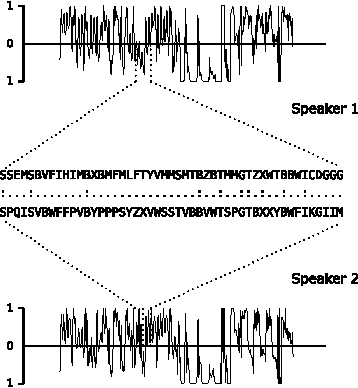
\includegraphics[width=\textwidth]{Body/Images-chap4/voice.pdf}

            %\scalebox{0.80}{
            %   \footnotesize
            %   \psset{xunit=1cm,yunit=1cm}
\readdata{\dataA}{Figures/voiceSeq1-xy.dat}
\readdata{\dataB}{Figures/voiceSeq2-xy.dat}
\begin{pspicture}(0,0)(10,10)%\showgrid
	\rput(2,9){
		\rput(-1,0){
			\psaxes[tickstyle=bottom, dy=\psyunit,Dy=1,Oy=0,Ox=0,Dx=100](0,0)(0,-1)(8,1)
		}
		\dataplot[plotstyle=line,linecolor=black,linewidth=0.1mm]{\dataA}
	}
	\rput(2,1){
		\rput(-1,0){
			\psaxes[tickstyle=bottom, dy=\psyunit,Dy=1,Oy=0,Ox=0,Dx=100](0,0)(0,-1)(8,1)
		}
		\dataplot[plotstyle=line,linecolor=black,linewidth=0.1mm]{\dataB}
	}
	\rput[l](0.4, 5.5){\normalsize \texttt{SSEMSBVFIHIMBXBMFMLFTYVMMSMTBZBTMMGTZXWTBBWICDGGG}}
	\rput[l](0.4, 5){\normalsize \texttt{:...:.......:...............:..:..::.:..:..:.....}}
	\rput[l](0.4, 4.5){\normalsize \texttt{SPQISVBWFFPVBYPPPSYZXVWSSTVBBVWTSPGTBXXYBWFIKGIIM}}
	\rput(0, 0){
		\psline[linestyle=dotted](4,2)(0.55,4.3)
		\psline[linestyle=dotted](4.4,2)(10.6,4.3)
		\psline[linestyle=dotted](4.4,2)(4.4,1)
		\psline[linestyle=dotted](4.2,2)(4.2,1)
	}
	\rput(0, 0){
		\psline[linestyle=dotted](4,8)(0.55,5.7)
		\psline[linestyle=dotted](4.4,8)(10.6,5.7)
		\psline[linestyle=dotted](4,8)(4,9)
		\psline[linestyle=dotted](4.4,8)(4.4,9)
	}
	\rput[bl](8.5, 8){Speaker 1}
	\rput[tl](8.5, 2){Speaker 2}

		
		
%	\rput(0.8,150){
%		\rotatebox{90}{ \# sequences}
%	}
%	\rput(8.5,150){
%		\rotatebox{-90}{ \# patterns}
%	}
%	\rput(5,0){
%		bootstrapping iterations
%	}


%	number LSWBBTTTTYZXBW SSEMSBVFIHIMBXBMFMLFTYVMMSMTBZBTMMGTZXWTBBWICD
%	       .............. :...:.......:...............:..:..::.:..:..:..
%	number TZXYSMFPYVVVTS SPQISVBWFFPVBYPPPSYZXVWSSTVBBVWTSPGTBXXYBWFIKG
%	250       260       270       280       290       300

%	310       320       330       340       350       360
%	number GGGCIWYFMELKKFTKPLILAAAAAAAAAADWZIHWIDDCCDNRAAAAAAAAAAAAAAAA
%	       ....................:::::::::...... ........::::::::::::::::
%	number IIMKPFIILHGDMSYTIEHEAAAAAAAAARITBTDEMGQEHCRAAAAAAAAAAAAAAAAA

\end{pspicture}

            %   \normalsize
            %}
        \caption[A Voice alignment of the spoken--letter ``X'' recorded from two different speakers]{
            An alignment of the spoken--letter ``X'' recorded from two different speakers.
            The plots at the top and bottom are recordings for first and second
            speakers, respectively.  The breakout in the center shows a section of the protein
            projection of each recording and the alignment generated using FastA
            as described in the text.  This example was taken from the first speech
            recognition experiment.  In this case, the bottom recording was the top
            scoring alignment against the top recording.
        }
        \label{fig:voiceAlign}
        \end{figure}

        \begin{figure}[phtb]
        \centering
        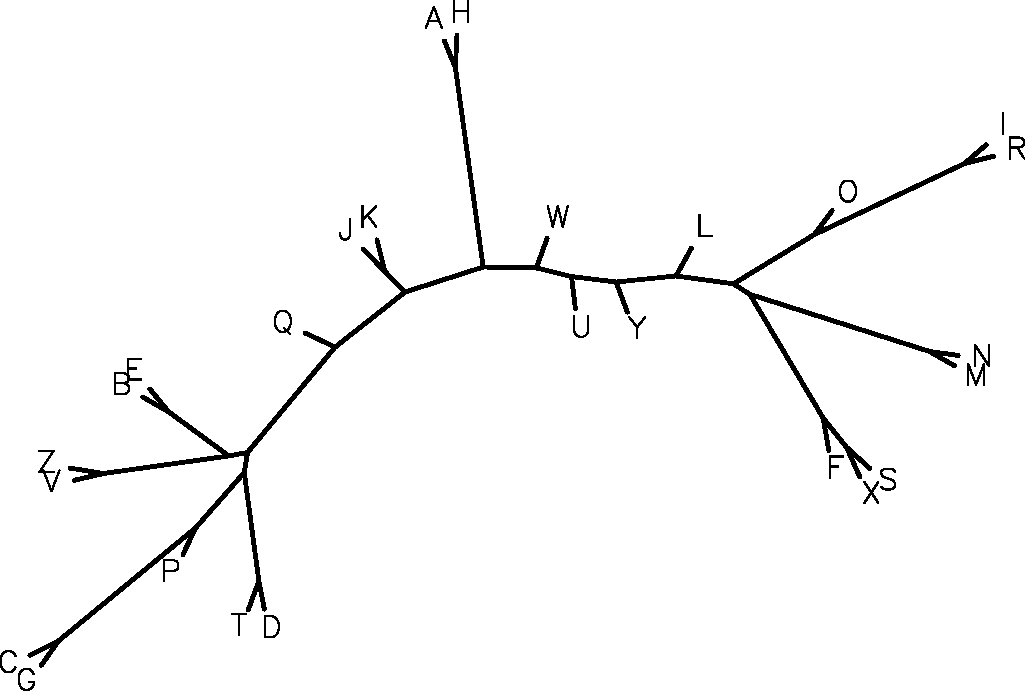
\includegraphics[width=\textwidth]{Body/Images-chap4/tree.pdf}
        \caption[A phylogenetic tree of voice--proteins]{
            A phylogenetic tree of voice--proteins.
            This tree was created using the
            Phylip~\cite{felsenstein1989phylip} tree drawing
            program from a multiple sequence alignment of
            all 26 voice--proteins from a single speaker.
            The multiple sequence alignment was made using the
            ClustalW~\cite{higgins1992improved} alignment tool,
            with the scoring matrix in Table~\vref{table:matrix}.
            In the tree, similar sounding (homologous) letters
            are grouped near each other.  For example, all the
            letters containing the /ee/ sound [\emph{B, C, D,
            E, G, P, T, V, Z}] are clustered on the left side
            of the tree.
        } \label{fig:tree} \end{figure}



\subsection{System and Methods}
    \subsubsection{Handwriting Recognition}
        For our handwriting recognition experiments, we used
        data from Alimoglu and Alpaydin, 1996, available in the
        University of California Irvine repository of machine
        learning databases~\cite{uci1998ucirepository}.  These data
        comprised of 10992 handwritten digits between \emph{0}
        and \emph{9}, written by 44 writers with each writer
        submitting 250 digits (8 samples were discarded by the
        original authors).

        Each digit was written with a stylus pen on a touch tablet,
        which recorded the $x$ and $y$ coordinates of the pen as a
        function of time.  These data were re-sampled such that each
        written digit was represented by a series of eight $(x,y)$
        points, spaced out by a constant arc length over the path of
        the digit.  Then, for each digit, the set of $(x,y)$ points
        were scaled such that the largest axis, usually the $y$ axis,
        ranged from 0 to 1.  By dividing the number line $[0,1]$
        into 23 ``bins'' we translated each of these coordinates
        into a pair of amino acids as shown in Figure~\vref{fig:pda}.
        We concatenated these amino acid pairs to obtain a protein
        sequence representation of each digit: a ``digit--protein.''




    \subsubsection{Speech Recognition}
        For our speech recognition experiments, we used data from
        Deitterich and Bakiri, 1995, %~\cite{dietterich1995solving}
        available in the University of California Irvine repository
        of machine learning databases~\cite{uci1998ucirepository}.
        This data set consisted of 7797 recordings of individuals
        speaking one of the letters \emph{A--Z}.  A total of 150
        speakers each said every letter \emph{A--Z} twice (three
        recordings were discarded by the original authors).
        Then, each recording was processed into a set of 617
        real--valued attributes in the range $[-1,1]$.  A more
        detailed description of the database is available from
        Dietterich \& Bakiri, 1995.%~\cite{dietterich1995solving}.

        By dividing the number line $[-1,1]$ into 23 bins we translated these real numbers into a series
        of amino acids.  For example, the series ``-1.0,-0.55, 0.11, 0.65'' was translated
        to ``{\texttt{AQKY}}''.  We concatenated these amino acids to make a protein representation
        of each recording: a ``voice--protein''.


\subsection{Results}
    \subsubsection{Handwriting Recognition}

        We conducted two handwriting recognition experiments.
        In both experiments part of the digit--protein database was assumed to contain a
        ``known'' set of digits that was subsequently used to annotate,
        or classify, the remaining ``unknown'' digits.  For our
        first experiment, we used for the known database containing the
        writing of 30 persons (7494 digits) and an unknown database
        with the writing of the remaining 14 persons (3498 digits).
        Using FastA, we searched each sequence from the unknown
        set in the known set and used the top scoring hits to
        annotate the unknown digits.  Searches were carried out
        using the scoring matrix shown in Table~\vref{table:matrix}
        with FastA version 3.4t11 using the default gap open and
        extension penalties, and the following options: \texttt{-p
        -Q -d0 -f-8 -g-1 -H -E1000 -b1}.  An example alignment of
        two handwritten nines from different writers is shown in
        Figure~\vref{fig:pdaAlign}.


        For our second experiment, we used 25\% (2748 digits) of our
        digit--protein database, selected randomly, as the unknown
        set and the remaining 75\% (8244 digits) as our known set.
        Alignments and annotations using FastA were performed as
        in the first experiment.

        The results of the two handwriting recognition
        experiments are shown in Table~\vref{table:results1}.
        In experiment 1, our results are about the same as
        the best k--means clustering results of Alimoglu and
        Alpaydin~\cite{alimoglu1996methods,alimoglu1997combining}.
        This experiment simulates the user--independent
        handwriting recognition problem: the handwriting of one
        group of writers was used to classify digits from a different group.
        In the user--dependent problem, experiment 2, the database
        of known handwritten digits contains samples from all the writers,
        on average.  Thus, for every unknown handwriting sample,
        there is often a close match in the database of known
        samples.  As such, the results of experiment 2 are
        significantly better than those of experiment 1 as shown
        in Table~\vref{table:results1}.



        %In contrast to k--means clustering and other common machine learning techniques for handwriting
        %recognition, there was no explicit training or learning phase of our experiments.  As such,
        %we included experiment 3, which is a realistic approximation of the recognition problem
        %on a tablet PC with multiple users.  The results for this experiment are considerably better than
        %experiment 2 because there are relatively more known sequences which can be used for annotating
        %the unknown sequence.

        In experiment 1, the average time for each alignment was
        0.117 seconds per unknown sequence on a 1 gHz Pentium III
        processor.  This is much shorter than the time required to
        write the digits.  Thus sequence alignment could be used
        as a ``real--time'' method for handwriting recognition.
        This high speed, together with the high accuracy for
        user--dependent recognition makes sequence alignment good
        candidate for use on a Tablet PCs, or even PDAs.

    \subsubsection{Speech Recognition}


        Using the voice--protein database, we conducted two
        experiments, analogous to the two handwriting recognition
        experiments described previously.  First, we used a known
        set consisting of 6238 recordings from 120 speakers and
        an unknown set with 1559 recordings from the remaining 30
        speakers.  Second, we used 25\% (1949 recordings) of the
        voice--protein database, selected randomly, as the unknown
        set and the remaining 75\% (5848 recordings) as the known
        set.  Each of the speech recognition alignments was performed
        using the same scoring matrix and FastA parameters as the
        handwriting recognition experiments.  An example alignment
        of two voice--proteins is shown in Figure~\vref{fig:voiceAlign}.


        The results of the two speech recognition experiments are shown in
        Table~\vref{table:results2}.
        Experiment 1 is compared
        to the best Error Correcting Output Code (ECOC) results of Deitterich
        and Bakiri~\cite{dietterich1995solving},
        but
        there was no comparison available for experiment 2.
        The misclassification for experiment 1 was 6.16\%,
        higher than the ECOC result of 3.27\%.  However, we observed that
        most of the errors were due to rhyming letters, and in particular
        all of the /ee/ sounding characters [\emph{B, C, D, E, G, P, T, V, Z}].
        This indicated that these characters were similar on a sequence level,
        so we constructed a phylogenetic tree of the sequences to study their
        relationship.



        A phylogenetic tree of 26 voice--proteins from a single
        speaker is shown in Figure~\vref{fig:tree}.  As the figure
        shows, the protein projections of phonetically similar
        letters tend to be homologous.  Furthermore, letters such
        as \emph{A} and \emph{H}, which have the /ay/ sound at the
        beginning, are more closely related to each other than
        they are to \emph{J} and \emph{K}, which have the /ay/
        sound at the end.  Because the /ee/ sounding letters all
        have /ee/ at the end, they are particularly difficult
        to distinguish from each other.  These letters account
        for a disproportionate majority of the errors in our two
        experiments.  By clustering these letters together such that
        they are considered the same for classification purposes,
        the error in experiment 1 was reduced to 1.09\%.  If the
        original error was evenly distributed between the classes,
        the error would have been reduced only to about 5.5\%.
        This suggests that, although string alignment performs
        poorly for /ee/ sounding characters, it performs well for
        all other characters.


\subsection{Conclusions}
        This work showed that sequence alignment can be a powerful
        classification tool for problems outside the domain
        of bioinformatics.  In both the handwriting and speech
        recognition problems, we projected real--valued data into
        strings of amino acids and used FastA as a classification
        tool, in a manner analogous to protein annotation.  In the
        case of handwriting recognition, we showed that sequence
        alignment is a viable alternative to traditional methods,
        such as k--means clustering, and is fast enough to be used
        as a real--time recognition method.


        There are many ways to improve upon the results we presented here.
        First, we did not have any explicit training phase for either set of experiments.
        However, there are at least two sequence alignment parameters which can
        be trained: the gap open and extension penalties, and the scoring matrix.
        The optimization of these parameters for protein annotation is well documented
        ~\cite{henikoff1993performance,altschul1991amino,henikoff1992aminoacid,dayhoff1979amodel,vogt1995assessment,henikoff2000amino}
        and would be similar for alternative sequence alignment applications such
        as handwriting recognition.  Second, intelligent projection of data
        into strings can greatly improve results.  Here, we used bins of equal
        size to partition the real--valued data into amino acids; however, bins
        of unequal size may improve the resolution between closely related sequences
        and improve classification.  Finally, more customizable sequence alignment tools
        would be very useful.  These tools should take an arbitrary alphabet (Blast
        and FastA are restricted to 23 amino acids) and a user--defined scoring
        matrix (FastA allows user--defined matrices, but Blast does not).

        The potential applications of sequence alignment tools
        outside of bioinformatics are boundless.  Tools such as Blast
        and FastA can be used to quickly classify or search through
        any data that can be projected into a string of characters.
        Of course, these methods will work best with data that is
        of a low dimension.  Our experiments with more complex data
        data, such as color images, suggest that how the data are
        projected into a string is very important with large number
        of dimensions.  However, for simple types of data, such
        as customer purchase histories, black and white images, or
        Internet chat transcripts, we have been able to use sequence
        alignment as a quick and effective classification tool.

\clearpage
\section{Machine learning approaches to modeling the physiochemical properties of
peptides}

% The very first letter is a 2 line initial drop letter followed
% by the rest of the first word in caps.
%
% form to use if the first word consists of a single letter:
% \PARstart{A}{demo} file is ....
%
% form to use if you need the single drop letter followed by
% normal text (unknown if ever used by IEEE):
% \PARstart{A}{}demo file is ....
%
% Some journals put the first two words in caps:
% \PARstart{T}{his demo} file is ....
%
% Here we have the typical use of a "T" for an initial drop letter
% and "HIS" in caps to complete the first word.
\subsection{Introduction}
In this section, I discuss the modeling of small peptide sequences
using non--grammatical models. Most commonly, peptides and protein
sequences are represented as a string of letters drawn from the
alphabet of characters representing the twenty natural amino acids.
Here, I present a series of experiments using a more meaningful
representation of amino acids and test the ability of various
machine learning techniques to predict peptide function.
Specifically, I develop a set of three amino acid representation
schemes and test these schemes combinatorially with a set of six
machine learning techniques. All of the work described in this
section
    is part of a publication appearing in the proceedings of the fourth
    Singapore--MIT Alliance Programme on Molecular Engineering of Biological and Chemical
    Systems, which was co--authored with Mark Styczynski and Gregory Stephanopoulos.
    Throughout this section, the use of the pronoun ``we'' refers to
    these authors.

\subsection{Motivation and background}

\subsubsection{Amino acid representations}
The most common representation of small peptides are as strings of
letters representing the twenty amino acids, e.g. \texttt{KWRAG},
which is the five residue sequence lysine, tryptophan, arginine,
alanine, and glycine.  Notably, both amino acid names and their
corresponding abbreviations are human constructs that carry no
information about the underlying physiochemical characteristics of
each amino acid.  That is, the string \texttt{KWRAG} carries little
information in and of itself, without some information about what a
\texttt{K} is and how it is different from the other amino acids.
In place of such physical descriptions, previous efforts have
described the similarity of amino acids based on the tendency for
one amino acid to substitute for another in homologous,
similarly--functioning proteins across different
species~\cite{henikoff1992aminoacid,dayhoff1979amodel}. That is,
substitutions that are observed in nature can be construed in some
sense as indicating similarity between certain amino acids. While
such efforts have been extremely useful for tasks such as aligning
more distant protein homologs, they typically do not capture enough
information to be practically useful in \textit{de novo} design or
prediction of protein activity.

Here we experiment with feature vector representations of small
peptides using sets of amino acid physiochemical characteristics
derived from the AAindex
database~\cite{kawashima1999aaindex,tomii1996analysis,nakai1988cluster}.
The AAindex database lists 453 physiochemical parameters for each of
the twenty amino acids.  These parameters range from those that are
very tangible and intuitive --- for example, residue volume, which
is AAindex parameter BIGC670101~\cite{bigelow1967on} --- to the
abstract --- for example, the normalized frequency of participation
in an N-terminal beta--sheet, which is AAindex parameter
CHOP780208~\cite{chou1978prediction}.  The parameters were culled
from the scientific literature by the AAindex authors and might be
considered the universe of what we, as the scientific community,
know about each amino acid.

Thus, a very logical way of representing an amino acid is as a
feature vector of these 453 attributes.  In this sense each type of
amino acid has a different feature vector of the same
dimensionality.  This might be considered the ``maximally
informative'' representation of the amino acids since it
incorporates an expansive set of features culled from the
literature.  Extending this, we could write an amino acid sequence
as the concatenation of these vectors.  That is, a three residue
peptide could be represented as a $3*453=1359$ feature vector.
Intuitively, this representation retains more information than the
string representation.  Further, we would imagine that the
physiochemical representation would be more useful for modeling the
function of a peptide sequence, such as its propensity to fold in a
certain manner or to react with a certain enzyme.

The representation of amino acids has received some previous
attention in the literature.  For example, Atchley \emph{et.\
al.}~\cite{atchley2005solving} use the physiochemical parameters
from the AAindex to create a low--dimensional projection of the
characteristics of each of the twenty natural amino acids.  Further,
they used this low--dimensional progression to derive metrics of
similarity between the amino acids, similar to popular amino acid
scoring matrices such as Blosum~\cite{henikoff1992aminoacid} and
PAM~\cite{dayhoff1979amodel}.


%\cite{buck2005networks}
%\cite{grantham1974amino}
% needed in second column of first page if using \pubid
%\pubidadjcol

\subsubsection{HIV--I Protease}
In this work we will use the HIV--I protease as a model system for
demonstrating the merits of different physiochemical amino acid
representations.  Specifically, we show the success of different
representations and different machine learning methods at modeling
substrate specificity of the protease.

The HIV--1 protease is a proteolytic enzyme encoded by the HIV
genome~\cite{brik2003hiv}.  The protease plays a critical role in
viral replication and the development of viral
structure~\cite{wang2001computational}. The protease recognizes
specific eight--residue sequences in its substrates (see
Figures~\vref{fig:hiv1p} and~\vref{fig:pockets}).  The protease's
natural targets are subsequences of other HIV genes which must be
cleaved for the virus to successfully replicate.  Accordingly, small
molecule inhibitors of the protease are a common therapy for
HIV/AIDS~\cite{boden1998resistance}.

    \begin{figure}[phbt]
    \centering
    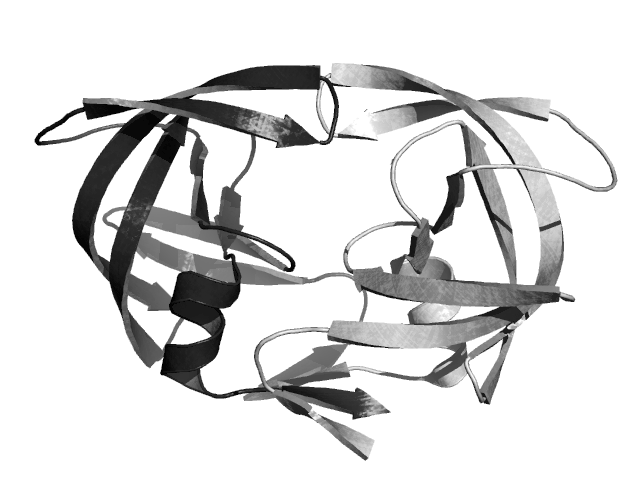
\includegraphics[width=2.5in]{Body/Images-chap4/hiv1p.png}
    \caption[Structure of the HIV--I protease,
    derived from the Protein Data Bank
    (PDB)~\cite{berman2000protein} entry 7HVP~\cite{swain1990x-ray}]{Structure of the HIV--I protease,
    derived from the Protein Data Bank
    (PDB)~\cite{berman2000protein} entry 7HVP~\cite{swain1990x-ray}.
    Over one hundred other structures of the protease
    have been solved since the first in 1989 and are
    available from the PDB's website.  The protein is
    a dimer of two 99 amino acid chains.  The regions
    of the protein at the top of the figure, the
    ``flaps,'' open up and accept a substrate protein,
    closing behind it.  Two aspartate residues in the
    active site, aided by the presence of water,
    act to cleave the substrate.} \label{fig:hiv1p}
    \end{figure}

    \begin{figure}[phbt]
    \centering
    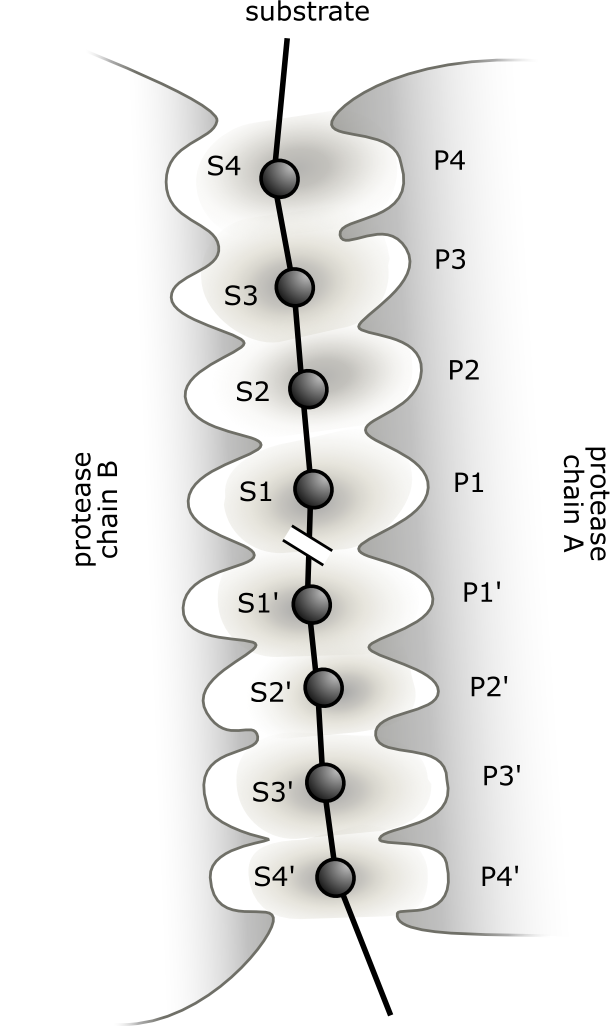
\includegraphics[width=2.0in]{Body/Images-chap4/pockets.png}
    \caption[Schematic of the HIV--I protease active site]{Schematic of the HIV--I protease active site.
    The active site comprises eight binding pockets (P1--P4
    and P1'--P4') into which eight residues from the
    target protein fall.  The target protein is cleaved between
    the S1 and S1' residues.  One half of the catalytic
    unit is made up by chain A of the protease and the
    other by chain B (see Figure~\vref{fig:hiv1p}).
    }
    \label{fig:pockets}
    \end{figure}

In addition to the handful of sites that the protease cleaves to
facilitate viral development, it can cleave a number of other
``non--natural'' substrates~\cite{beck2002defining}.  These
substrates have been the focus of intense experimental
study~\cite{beck2000identification,bagossi2005amino,beck2001molecular,
clemente2004comparing}.  In a recent manuscript, You \emph{et.\
al.}\ collected a comprehensive set of 700+ eight--residue
substrates that have been tested for cleavability by the HIV--I
protease~\cite{you2005comprehensive}.  In addition, You \emph{et.\
al.}\ developed a series of models for the protease's substrate
selectivity that, in general, outperform previous computational
models~\cite{cai2002support,chou1996prediction,narayanan2002mining,rognvaldsson2004why},
which relied on a much smaller dataset~\cite{cai1998artificial}.


%\cite{brown2000knowledge-based}
%\cite{callebaut1996inhibition}


\subsection{Methods}

\subsubsection{Amino acid representations and input
data set} A set of 746 eight--residue peptides were generously
provided by You \emph{et. al.}\ ~\cite{you2005comprehensive}, each
with a class: cleavable by the HIV--I protease or not cleavable.  In
addition, the complete set of 453 physiochemical parameters for each
of the 20 naturally occurring amino acids was downloaded from the
AAindex database (release 7.0, July 2005).

From these 453 parameters, we removed redundant parameters for which
the magnitude of the correlation coefficient with another parameter
was greater than 0.80. The remaining 155 independent parameters were
kept.  Using these parameters, we made three different projections
of the 746 experimentally tested protease substrates as detailed
below.

\paragraph{Full physiochemical projection}
In this projection each eight--residue peptide was represented as a
1241--dimensional feature vector: 8 residues with 155 physiochemical
features per residue plus the class --- cleaved or not cleaved.  Of
our three representations, this one retains the most information
about the peptides.

\paragraph{Feature--selected physiochemical projection}
Using the ``FULL'' projection (above) we performed a feature
selection routine to select only those features that are most
correlated to the class.  (Throughout this manuscript, all modeling
and feature selection were performed using the Waikato Environment
for Knowledge Analysis, or WEKA ~\cite{witten2005data}).  Briefly,
we evaluated the worth of a subset of features by considering the
individual predictive ability of each feature with respect to the
cleaved/uncleaved class, along with the degree of redundancy between
the features.  Using this method, we created a 54--dimensional
projection of the peptide substrates (53 features plus the class).

Analysis of this lower--dimensional projection revealed that the
features of the outer residues (S4, S4') are relatively unimportant,
whereas the central residues (S1, S1') are quite important in
determining cleavability. For the S1 position, seven parameters were
chosen:
\begin{itemize}
    \item   FASG760102: Melting point~\cite{fasman1976handbook};
    \item   FAUJ880105: Minimum width of the side
        chain~\cite{fauchere1988amino};

    \item   PALJ810111: Normalized frequency of beta--sheet
        in alpha+beta class~\cite{palau1982protein};

    \item   PRAM900101: Hydrophobicity~\cite{prabhakaran1990distribution};

    \item   ROBB760107: Information measure for
        extended without H-bond~\cite{robson1976conformational};

    \item   KOEP990101: Alpha--helix propensity derived
        from designed sequences~\cite{koehl1999structure-based}; and

    \item   MITS020101: Amphiphilicity
        index~\cite{mitaku2002amphiphilicity}.
\end{itemize}

\paragraph{PCA projection of physiochemical properties}
Using the full, 155--dimensional representation of each of the 20
naturally occurring amino acids, we performed principal component
analysis (PCA) to find linear combinations of features that capture
the variation between different kinds of amino acids.  More
formally, PCA, or the Karhunen--Lo\`{e}ve transform, is a linear
transformation by which the 20 data points in a 155--dimensional
space are projected onto a new coordinate system.  The system is
chosen such that the greatest variance is captured by the first
axis, or the first ``principal component.''  Successive principal
components (axes) capture progressively less variance.  Each
component is a linear combination of some of the initial features;
given appropriate uniform normalization, the weight of each feature
in a given component indicates the relative importance of that
feature in defining the component.

Using PCA, we derived 16 principal components that capture 95\% of
the variance in the amino acids, with the first PC capturing 30\% of
the variance.  The set of 746 peptide 8--mers were projected into a
reduced 129--dimensional space: 8 concatenated 16--dimensional
residues plus the class of the peptide.


\subsubsection{Model creation and classification}
For each of the three peptide representations detailed above, we
tested the ability of six machine learning techniques to classify
the peptides as either cleaved or uncleaved.  Each of these models
is described below. For each model, we evaluated the performance
using 10x10 cross--validation (see Conclusion): for each of ten
runs, 10\% of the peptide dataset was withheld for testing a
classifier trained by the remaining 90\% of the peptides. The
sensitivity and specificity of each classifier's predictions for all
ten of its cross--validation runs can then be combined to determine
the percentage of correctly classified peptides.  This value is used
to quantify the classifier's overall accuracy and facilitates
pairwise comparison of models and representation schemes.

\paragraph{Decision tree model}
Decision trees are simple, intuitive classification schemes that use
a series of questions (decisions) to place a sample in a class with
low error rate. More specifically, a decision tree is a structure in
which the internal branches represent conditions, such as
``hydrophobicity index at S3 $> 0.52$''.  Following these conditions
leads to the leaves of the tree, which are classifications
indicating whether the peptide is cleaved or not.  Here, we use a
particular variant of the decision tree, a C4.5 decision
tree~\cite{quinlan1992c4}, which is notable for not being prone to
overfitting of input data.  An example decision tree from our
experiments is shown in Figure~\vref{fig:decisionTree}.

   \begin{figure}[!h]
    \centering
    %\includegraphics[width=2.5in]{Images/barChart.pdf}
    \tiny
    \begin{verbatim}
CHOP780207_S2' <= 0.41765
|   FAUJ880105_S1 <= 0.57778
|   |   FASG760102_S1 <= 0.27711: uncleaved (32.0/1.0)
|   |   FASG760102_S1 > 0.27711
|   |   |   QIAN880122_S4' <= 0.81022
|   |   |   |   PRAM900101_S1 <= 0.27463
|   |   |   |   |   MEEJ810102_S4 <= 0.33702
|   |   |   |   |   |   RACS820112_S2 <= 0.58621
|   |   |   |   |   |   |   ZIMJ680101_S1' <= 0.52117
|   |   |   |   |   |   |   |   PRAM820101_S2' <= 0.43367
|   |   |   |   |   |   |   |   |   ROSM880103_S3' <= 0.23077: cleaved (2.0)
|   |   |   |   |   |   |   |   |   ROSM880103_S3' > 0.23077
|   |   |   |   |   |   |   |   |   |   CHOP780207_S4 <= 0.21176: cleaved (2.0)
|   |   |   |   |   |   |   |   |   |   CHOP780207_S4 > 0.21176: uncleaved (11.0/1.0)
|   |   |   |   |   |   |   |   PRAM820101_S2' > 0.43367
|   |   |   |   |   |   |   |   |   RADA880105_S2 <= 0.75274
|   |   |   |   |   |   |   |   |   |   PRAM900101_S1 <= 0.06866: cleaved (10.0/2.0)
|   |   |   |   |   |   |   |   |   |   PRAM900101_S1 > 0.06866: uncleaved (4.0)
|   |   |   |   |   |   |   |   |   RADA880105_S2 > 0.75274
|   |   |   |   |   |   |   |   |   |   QIAN880137_S3' <= 0.5124: cleaved (69.0/3.0)
|   |   |   |   |   |   |   |   |   |   QIAN880137_S3' > 0.5124
|   |   |   |   |   |   |   |   |   |   |   RACS820112_S2 <= 0.43103: cleaved (2.0)
|   |   |   |   |   |   |   |   |   |   |   RACS820112_S2 > 0.43103: uncleaved (4.0/1.0)
|   |   |   |   |   |   |   ZIMJ680101_S1' > 0.52117: cleaved (248.0/7.0)
|   |   |   |   |   |   RACS820112_S2 > 0.58621
|   |   |   |   |   |   |   RACS820103_S4 <= 0.43007
|   |   |   |   |   |   |   |   CHAM830104_S3' <= 0
|   |   |   |   |   |   |   |   |   RADA880105_S2 <= 0.75274: uncleaved (5.0/1.0)
|   |   |   |   |   |   |   |   |   RADA880105_S2 > 0.75274: cleaved (2.0)
|   |   |   |   |   |   |   |   CHAM830104_S3' > 0: cleaved (11.0)
|   |   |   |   |   |   |   RACS820103_S4 > 0.43007: uncleaved (6.0)
|   |   |   |   |   MEEJ810102_S4 > 0.33702
|   |   |   |   |   |   GARJ730101_S4' <= 0.01426: uncleaved (9.0)
|   |   |   |   |   |   GARJ730101_S4' > 0.01426
|   |   |   |   |   |   |   CHAM830104_S3' <= 0
|   |   |   |   |   |   |   |   QIAN880102_S4 <= 0.57143: uncleaved (7.0/1.0)
|   |   |   |   |   |   |   |   QIAN880102_S4 > 0.57143: cleaved (3.0)
|   |   |   |   |   |   |   CHAM830104_S3' > 0: cleaved (9.0)
|   |   |   |   PRAM900101_S1 > 0.27463
|   |   |   |   |   GEIM800106_S1' <= 0.94
|   |   |   |   |   |   RACS820102_S3 <= 0.81522
|   |   |   |   |   |   |   FAUJ880108_S2' <= 0.4375: uncleaved (31.0/1.0)
|   |   |   |   |   |   |   FAUJ880108_S2' > 0.4375: cleaved (4.0/1.0)
|   |   |   |   |   |   RACS820102_S3 > 0.81522: cleaved (6.0)
|   |   |   |   |   GEIM800106_S1' > 0.94: cleaved (9.0)
|   |   |   QIAN880122_S4' > 0.81022
|   |   |   |   MITS020101_S1 <= 0.35354
|   |   |   |   |   ZIMJ680101_S1' <= 0.82085: uncleaved (20.0)
|   |   |   |   |   ZIMJ680101_S1' > 0.82085
|   |   |   |   |   |   RACS820102_S3 <= 0.3587: uncleaved (4.0)
|   |   |   |   |   |   RACS820102_S3 > 0.3587: cleaved (5.0)
|   |   |   |   MITS020101_S1 > 0.35354: cleaved (2.0)
|   FAUJ880105_S1 > 0.57778
|   |   QIAN880137_S3' <= 0: cleaved (3.0)
|   |   QIAN880137_S3' > 0: uncleaved (37.0/1.0)
CHOP780207_S2' > 0.41765
|   ZIMJ680101_S1' <= 0.58306: uncleaved (145.0/2.0)
|   ZIMJ680101_S1' > 0.58306
|   |   PRAM900101_S1 <= 0.27463
|   |   |   FAUJ880105_S1 <= 0.57778
|   |   |   |   FAUJ880105_S1 <= 0: uncleaved (2.0)
|   |   |   |   FAUJ880105_S1 > 0
|   |   |   |   |   RACS820103_S3 <= 0.72378
|   |   |   |   |   |   WILM950104_S2 <= 0.44834: uncleaved (5.0)
|   |   |   |   |   |   WILM950104_S2 > 0.44834
|   |   |   |   |   |   |   PRAM820101_S2' <= 0.77041: cleaved (8.0)
|   |   |   |   |   |   |   PRAM820101_S2' > 0.77041: uncleaved (4.0/1.0)
|   |   |   |   |   RACS820103_S3 > 0.72378: cleaved (9.0)
|   |   |   FAUJ880105_S1 > 0.57778: uncleaved (4.0)
|   |   PRAM900101_S1 > 0.27463: uncleaved (12.0)
    \end{verbatim}
    \caption[Decision tree calculated for modeling 8--mer peptides]{The decision tree calculated for the
    CFS, a 54--dimensional representation of the 8--mer
    peptides.  The branch points are in the form
    PARAMETER\_RESIDUE\@.  For example, \texttt{CHOP780207\_S2'}
    represents the AAindex parameter \texttt{CHOP780207}
    (normalized frequency of participation in a C--terminal non--helical
    region) at the S2' residue.  Values for all
    AAindex parameters are normalized to 1 across all
    amino acids.  The tree shows various questions
    about a peptide that, when followed, lead to a
    set of conclusions.   For example, if 
    a given peptide has
    \texttt{CHOP780207\_S2 <= 0.41765} and
    \texttt{FAUJ880105\_S1 > 0.57778} and
    \texttt{QIAN880137\_S3 > 0} then the peptide
    is classified as uncleaved.  As shown in the
    table, 37 of the 746 known peptides are
    correctly classified
    by this scheme and only one is incorrectly
    classified.
    } \label{fig:decisionTree}
    \end{figure}


\paragraph{Logistic regression model}
A logistic regression is just a non--linear transformation of a
linear regression.  In this model, each independent variable (the
different dimensions of our various projections) are regressed to
the class (cleaved or not cleaved).  Here we use a variant of
logistic regression that leads to automated feature selection and is
described elsewhere~\cite{landwehr2003logistic}.

\paragraph{Bayesian network model}
Bayesian network models use directed acyclic graphs to model the
joint probability distribution of each class over all input
features. That is, the model captures conditional dependencies
between the features with regards to how they impact the final
classification of each sample.  Bayesian networks can be used to
find causality relationships, one of many features that make these
models particularly well--suited to many applications in
computational biology (see, for
example,~\cite{scott2004predicting,hartemink2002bayesian,friedman2000using}).
The method uses a Bayesian scoring metric that ranks multiple models
based on their ability to explain data with the simplest possible
method.  The Bayesian metric is a function of the probability of the
model being correct given a set of observed data; this is, in turn,
correlated to the model's prior probability and its physical
likelihood. For a more detailed explanation of Bayesian networks,
see Witten and Frank~\cite{witten2005data} or
Heckerman~\cite{heckerman95tutorial}.

\paragraph{Naive Bayes model} The naive Bayes model, or ``Idiot's''
Bayes model~\cite{hand2001idiots}, is a simple machine learning
scheme that assumes \emph{naively} that each feature has an
independent effect on the classification of each
sample~\cite{john1995estimating}.  In the case of the HIV--I
protease substrates, this means that the physiochemical
characteristics of the S1 residue contribute to the cleavability of
the peptide in a way that is independent of the other residues: S1',
S2, etc.  The resulting network dependencies are less complex than
one might otherwise obtain from a Bayesian network model but are
frequently useful, particularly for unwieldy datasets or problems
with physical characteristics that may warrant the assumption of
conditional independence of features.

\paragraph{Support vector machine model with linear basis function}
The support vector machine (SVM) is a machine learning technique
posed as a quadratic programming (QP)
problem~\cite{bennett2000support}. The formulation can best be
conceptualized by considering the problem of classifying two
linearly separable groups of points.  The first step is to define
the ``convex hull'' of each group, which is the smallest--area
convex polygon that completely contains a group.  The SVM approach
looks for the best linear classifier (single straight line) between
the two groups of points, defined as either the line that bisects
the two closest points on each convex hull or the two parallel
planes tangent to each convex hull that are furthest apart.  These
alternative definitions provide two alternative formulations of a
convex QP problem; notably, they both reduce to the same problem.
(A rigorous mathematical treatment of these qualitative explanations
can be found
elsewhere~\cite{bennett2000duality,crisp1999geometric}.) Tried and
true methods for solving QP problems can then be used to (relatively
quickly) determine the best classifier.  This method can be expanded
to allow for linearly inseparable cases by altering the optimization
problem to account for a weighted cost of misclassification when
training the model.  There is evidence in the literature that an SVM
approach to defining the best classifier is less susceptible to
overfitting and generalization
error~\cite{cristianini2000introduction,vapnik1998statistical,vapnik1995nature}.

\paragraph{Support vector machine model with radial basis function}
The above description of an SVM, despite accounting for the
possibility of inseparability, does not address the need for
non--linear classifiers. For instance, if the members of one class
fall within a well--defined circle and the non--members fall outside
of the circle, the above method will perform extremely poorly
because it will try to form just one plane to separate the
groups~\cite{bennett2000support}.  Rather than attempting to fit
higher--order curves, it is easier to project the input attributes
into a higher--dimensional space in which the groups are
(approximately) linearly separable.  The higher--dimensional spaces
can be characteristic of any desired classifier (e.g., nonlinear
terms generated by multiplying attributes or squaring attributes).
The same method for computing the best linear classifier is then
used.   The result is mapped back into attribute space of the
appropriate dimensions and constitutes a non--linear classifier.
Though one may expect such a process to be prohibitively expensive
for data with many attributes, there exists a computational shortcut
using ``kernel functions'' to avoid calculating all possible
higher--dimensional feature values.  In this work, the basis
function for the kernel gives us the ability to detect optimal
classifiers that are based upon training points' radius from some
center point (as in the above example).



\subsection{Conclusion}
    Our results show that the full, 1241--dimensional
    representation performed the best, followed by the PCA
    representation and, finally, the representation made
    via feature selection.  (See Figure~\vref{fig:barChart}
    and Table~\vref{table:repComp} \&~\vref{table:repRank}.
    In these tables ``FULL'' is the full physiochemical,
    1241--dimensional representation; ``CFS'' is the
    feature--selected, 55--dimensional representation; and
    ``PCA'' is the 129--dimensional representation
    created using principal component analysis.)

    \begin{figure}[phbt]
    \centering
    \includegraphics[width=2.5in]{Body/Images-chap4/barChart.pdf}
    \caption[Classification results for all
    amino acid representations and model types]{Classification results for all
    amino acid representations and model types.
    The three different amino acid representations
    are shown in shades of gray: ``FULL'' is the full
    physiochemical, 1241--dimensional representation;
    ``CFS'' is the feature--selected, 55--dimensional
    representation; and ``PCA'' is the 129--dimensional
    representation using created using princple
    component analysis (see text).  Error bars
    show the standard deviation over the
    10x10 cross--validation test (100 samples per
    representation/model combination with a total of
    1800 tests.)  The best performing model was the
    SVM with radial basis function (SVM--rbf in the
    figure) with the full 1241--dimensional feature
    vector representing each eight--residue sequence.
    Averaged over all representations, the logistic
    regression model is best (see Table~\vref{table:modelComp}).
    The poorest performing model is the decision tree
    (DT) with the 129--dimensional feature vector
    created using the PCA projections created as
    described in the text.  In general the full 1241--dimensional
    representation performed the best,
    followed by the PCA representation and finally
    the CFS representation, which was created by a
    feature selection process.  } \label{fig:barChart}
    \end{figure}

    Of the models tested, results show that logistic
    regression is the best, followed by (linear basis function) SVMs and
    Bayesian networks (See Figure~\vref{fig:barChart} and
    Table~\vref{table:modelComp} \&~\vref{table:modelRank}.)  The
    single best model/representation combination was the
    SVM model with radial basis function (SVM--rbf) and
    the FULL representation.  It is worth noting that though
    this single combination was the best, the radial basis function
    SVM itself did not perform consistently well.  Though this
    may not have been expected, it is definitely reasonable
    per the ``No Free Lunch'' theorem:
    no single machine--learning method should be expected to
    perform the best in all cases~\cite{wolpert1995no}.

    In general, these results suggest that
    higher--dimensional physiochemical representations
    tend to have better performance than representations
    incorporating fewer dimensions selected on the basis
    of high information content.  As such, it seems that
    as long as the training set is a reasonable
    size, more accurate classifiers can be constructed by
    keeping as many significant input attributes as possible.
    Though methods like principal
    components analysis help to reduce computational complexity
    for unwieldy datasets, it is better to avoid feature
    selection until a supervised method (like the models tested
    in this work) can determine which features are most important
    in classifying samples.

    \begin{table}
    \caption[Machine learning model comparison]{Machine learning model comparison.  Each $i,j$ entry represents the number of representations,
    out of three, for which the $i$ model performed \emph{worse} than the $j$
    model.  Here ``worse'' means that the model had a statistically significant
    lower performance, based on a two--tailed t--test at the 0.05 confidence level.}
    \label{table:modelComp}
    \centering
    \begin{tabular}{rcccccc} \hline \hline
        & DT & LR & NB & BN & SVM & SVM--rbf \\
        DT & - & 2 & 1 & 3 & 2 & 2 \\
        LR & 0 & - & 0 & 0 & 0 & 0 \\
        NB & 0 & 3 & - & 1 & 2 & 1 \\
        BN & 0 & 1 & 0 & - & 1 & 1 \\
        SVM & 0 & 0 & 0 & 0 & - & 1 \\
        SVM--rbf & 0 & 2 & 0 & 1 & 2 & - \\ \hline \hline
    \end{tabular}
    \vspace{12pt}


    \end{table}

    \begin{table}
    \caption[Machine learning model ranking]{Machine learning model ranking. Each row shows,
    for each model, how many other model/representation
    pairs that model (with any
    representation) ``wins'' against.  (Thus, the max of the sum
    of the columns in any row is $18-3=15$; however,
    ties are not shown.)  Here ``win/loss'' means
    that the model had a statistically significant
    higher/lower performance, based on a two--tailed
    t--test at the 0.05 confidence level.}\label{table:modelRank}
    \centering
    \begin{tabular}{ccc} \hline \hline
        total wins & total losses & model \\ \hline
       8 &  0 &  LR \\
       7 &  1 &  SVM \\
       5 &  3 &  BN \\
       5 &  5 &  SVM--rbf \\
       1 &  7 &  NB \\
       0 &  10 &  DT \\ \hline \hline
    \end{tabular}
    \vspace{12pt}
    \end{table}

    \begin{table}
    \caption[Machine learning representation comparison]    {Machine learning representation comparison.  Each $i,j$ entry represents the
    number of models, out of six, for which the $i$
    representation performed \emph{worse} than the
    $j$ representation.  Here ``worse'' means that
    the representation had a statistically significant
    lower performance, based on a two--tailed t--test
    at the 0.05 confidence level.}\label{table:repComp}
    \centering
    \begin{tabular}{rccc} \hline \hline
    & FULL & CFS & PCA \\
     FULL & - & 0 & 1  \\
     CFS & 3 & - & 4  \\
     PCA & 2 & 1 & -  \\ \hline \hline
    \end{tabular}
    \vspace{12pt}
    \end{table}

    \begin{table}
    \caption[Machine learning representation ranking]{Machine learning representation ranking. Each row shows, for each representation,
    how many other model/representation pairs that representation (with any
    model) ``wins'' against.  (Thus, the max of the sum
    of the columns in any row is $18-6=12$; however,
    ties are not shown.)  Here ``win/loss'' means
    that the representation had a statistically significant
    higher/lower performance, based on a two--tailed
    t--test at the 0.05 confidence level.}\label{table:repRank}
    \centering
    \begin{tabular}{ccc} \hline \hline
    5 & 1 & FULL \\
    5 & 3 & PCA \\
    1 & 7 & CFS \\ \hline
    \end{tabular}
    \vspace{12pt}

    \end{table}

\clearpage
\section{Identifying functionally important mutations from phenotypically diverse sequence data}
\subsection{Introduction}

In the previous section, I departed from the use of grammar--based
models of sequences and explored statistical modeling approaches.
This section continues this line of work, but is focused on the
identification of important mutations in nucleotide sequences,
rather than global, physiochemical characteristics of small
peptides.  In particular, in this section I present a simple
statistical method for parsing out the phenotypic contribution of a
single mutation from libraries of functional diversity that contain
a multitude of mutations and varied phenotypes. This work is part of
a publication that is in press at \emph{Applied and Environmental
Microbiology}, which was co--authored with Hal Alper, Curt Fischer,
and Gregory Stephanopoulos.  Throughout this section, the use of the
pronoun ``we'' refers to these authors.


\subsection{Motivation}

    The engineering of  functional nucleic acid sequences
    and other biomolecules is frequently hampered by a
    limited understanding of how specific mutations at
    a genotype level are manifested in the phenotype.
    For some well--studied, large protein families, these
    relationships can be inferred; however, such cases
    are rare.  In the absence of these relationships, we
    resort to strategies that explore the genotype space
    in a random manner, such as directed evolution.

    In many cases, directed evolution of genes
    and other functional DNA loci is an effective
    approach to sample the sequence space in search of
    biomolecules with desirable properties ~\cite{glieder2002laboratory,solem2002modulation}.
    However,  the most successful examples employ
    a selectable fitness criterion that allows for
    high-throughput screening of the mutational space:
    sampling a large enough space eliminates the need
    to make rational mutations.  For many proteins or
    functional nucleic acids, it may not be possible
    to link a desired phenotype with a selectable
    criterion, fit for high-throughput screening.
    In the absence of such a criterion, clonal
    populations of mutants must be assayed individually
    for the phenotype of interest.  This scenario
    might be called ``assay--based'' directed evolution,
    a situation in which the upstream mutagenesis
    has a higher throughput than the downstream
    characterization.  In this scenario, there is a
    premium on information linking mutational changes
    to their phenotypic manifestations.  Further,
    there is a strong incentive to ``learn from''
    the  (relatively small) mutational spectra of
    these mutants to determine sequence-phenotype
    interactions, and to use this information
    rationally in subsequent rounds of mutagenesis.

          Here, we present a simple statistical
          method for analyzing a mutational spectrum
          to parse out the phenotypic manifestation
          of individual mutations, even when they
          are masked by the presence of many other
          mutations.  Because assay-based directed
          evolution does not employ any pre--screening
          or selection of clones, as is the case
          when a selectable marker is available,
          mutants are expected to have a range of
          phenotypes, including both increased and
          decreased fitness.    Here, we demonstrate
          our method by identifying mutations in
          a library of mutagenized PL--$\lambda$ promoters
          ~\cite{alper2005tuning} that result in either  increased or
          decreased promoter activity and we show how
          to quantify the statistical confidence in
          these mutation-phenotype linkages

          The central premise of our method is that
          mutations that have no effect on mutant
          phenotype should partition randomly,
          following a multinomial distribution,
          between phenotypic classes.  For example,
          consider a hypothetical experiment in which
          we mutagenize a protein that can fluoresce
          in one of three colors: red, blue, or green.
          After generating a library of 1000 mutants,
          each bearing many point mutations, our assay
          reveals that 600 have the red phenotype,
          300 are blue, and 100 are green.  If  a
          particular point mutation has no effect on
          the color, then we expect that, by chance,
          mutants containing this modification will
          be distributed between the red, blue, and
          green classes in a ratio of 6:3:1.  That is,
          the mutation should not be correlated
          to any particular phenotypic class.
          More rigorously, we say that the mutations
          are multinomially distributed between the
          three classes with background frequencies
          0.6, 0.3, and 0.1.

          Multinomial statistics and related
          combinatorial statistics commonly arise
          in the analysis of naturally--occurring
          mutational diversity~\cite{adams1987statistical,piegorsch1994statistical}.  For example,
          similar statistical analyses have been
          used to find functional gene domains
          ~\cite{lossos2000inference}, important structural RNA sites~\cite{johnson2004selection},
          and genomic loci with an overabundance
          of single nucleotide polymorphisms (SNPs)
          ~\cite{walker1999evolutionary}.   Here we apply multinomial statistics
          to the analysis of an artificially generated
          mutational landscape to parse out critical
          residues controlling phenotypic behavior.
          We show that, based on this information,
          mutants with sets of individual mutations
          can be made, and we suggest that this can
          be used as a method for improving directed
          evolution experiments by incorporating
          sequence information.

        In what follows, we detail the construction
        of numerous PL--$\lambda$ promoter variants, which
        were generated by error--prone PCR such
        that each mutant incorporated many point
        mutations. The activity of these promoters
        was assayed using flow cytometry to measure
        the fluorescence of a GFP reporter gene.
        We show how our statistical analysis
        revealed the phenotypic manifestation
        of numerous mutations.  Finally, we
        present a validation of our method
        by constructing point mutations for
        several of the identified mutations and
        combinations of sites using site-directed
        mutagenesis.  These mutations, we show,
        have the predicted effect on the promoter
        phenotype, even when removed from the
        background of other mutations.

\subsection{Materials and Methods}


\subsubsection{Strains and Media}

\emph{E. coli} DH5$\alpha$ (Invitrogen) was used for routine
transformations as described in the protocol.  Assay
strains were grown at 37\textcelsius~with 225 RPM orbital
shaking in M9-minimal media (11)  containing 5 g/L
D--glucose and supplemented with 0.1\% casamino acids.
All other strains and propagations were cultured at
37\textcelsius~in LB media.  Media was supplemented with 68
$\mu$g/ml chloramphenicol.  All PCR products and restriction
enzymes were purchased from New England Biolabs and
utilized Taq polymerase.  M9 Minimal salts were purchased
from US Biological and all remaining chemicals were from
Sigma-Aldrich.



\subsubsection{Library Construction}

Nucleotide analogue mutagenesis was carried out in the presence of
20�$\mu$M 8--oxo--2'--deoxyguanosine (8--oxo--dGTP) and
6--(2--deoxy--$\beta$--D--ribofuranosyl)--3,4--dihydro--8H--pyrimido--[4,5--c][1,2]oxazin--7--one
(dPTP) (TriLink Biotech), using plasmid pZE--gfp(ASV) kindly
provided by M. Elowitz as template~\cite{lutz1997independent} along
with the primers PL\_sense\_AatII, TCCGACGTCTAAGAAACCATTATTATC and
PL\_anti\_EcoRI, CCGGAATTCGGTCAGTGCGTCCTGCTGAT. Ten and 30
amplification cycles with the primers mentioned above were
performed. The 151 bp PCR products were purified using the GeneClean
Spin Kit (Qbiogene). Following digestion with AatII and EcoRI, the
product was ligated overnight at 16\textcelsius~and transformed into
library efficiency \emph{E. coli} DH5$\alpha$ (Invitrogen). About
30,000 colonies were screened by eye from minimal media--casamino
acid agar plates and 200 colonies, spanning a wide range in
fluorescent intensity, were picked from each plate.  Selected
mutants were sequenced using primers PL\_Sense\_Seq,
\begin{equation*}
\texttt{AGATCCTTGGCGGCAAGAAA}
\end{equation*}
and PL\_Anti\_Seq,
\begin{equation*}
\texttt{GCCATGGAACAGGTAGTTTTCCAG}.
\end{equation*}



\subsubsection{Library Characterization}

About 20 $\mu$L of overnight cultures of library clones growing in
LB broth were used to inoculate 5mL M9G medium supplemented with
0.1\% w/v casamino acid (M9G/CAA). The cultures were grown at
37\textcelsius~ with orbital shaking. After 14 h, roughly the point
of glucose depletion, a culture sample was centrifuged at 18,000 g
for 2 minutes, and the cells were resuspended in ice--cold water.
Flow cytometry was performed on a Becton--Dickinson FACScan as
described elsewhere~\cite{alper2005tuning}, and the geometric mean
of the fluorescence distribution of each clonal population was
calculated.

Mean and standard deviation were calcuated from the FL1--H
distribution resulting after gating the cells based on a
FSC--SSC plot. A total of 200,000 events were counted to
gain statistical confidence in the results



\subsubsection{Construction of designed promoters}

Promoters with specific nucleotide changes were created
using overlap--extension PCR and primers specifically
designed to incorporate these changes.  Primers were
designed to divide the promoter region into thirds,
and the proper primers were assembled piecewise in a PCR
reaction consisting of 95\textcelsius~for 4 minutes, 10
cycles with an annealing temperature of 44\textcelsius,
followed by 30 cycles of PCR with an annealing temperature
of 60\textcelsius, and a final extension for 3 minutes at
72\textcelsius.  Fragments were gel extracted using 2.5\%
agarose gels and Qiagen MERmaid spin kit.  The isolated
fragment was then linked with the final primer using the
same PCR and extraction procedures.  Finalized fragments
were then digested using EcoRI and AatII and ligated into
the digested plasmid backbone.  Sequencing was performed
to verify correct constructs.



\subsection{Results}



\subsubsection{Generation of mutant library}

 Previously, we reported on the development of a promoter
 library generated through the random mutagenesis of the
 sequence space~\cite{alper2005tuning}.  In that work, library diversity was
 created through error--prone PCR of the  PL--TET01 promoter,
 a variant of the PL--$\lambda$ promoter~\cite{cirino2003generating}, which was placed
 upstream of a gfp gene.  The promoter region contains
 two tandem promoters  PL--1 and  PL--2, each of which
 contains -10 and -35 sigma factor binding sites~\cite{giladi1995enhanced,giladi1998participation,giladi1996identification}.
 Furthermore, the promoter contains, at approximately the
 same location, an UP element that binds C--terminal domain
 of the alpha subunit and a binding site for integration
 host factor (IHF).  In addition, the  PL--TET01 promoter
 has two tetO2 operators from the Tn10 tetracycline
 resistance operon~\cite{lutz1997independent}.

        \begin{sidewaysfigure}[ptb]
        \centering
        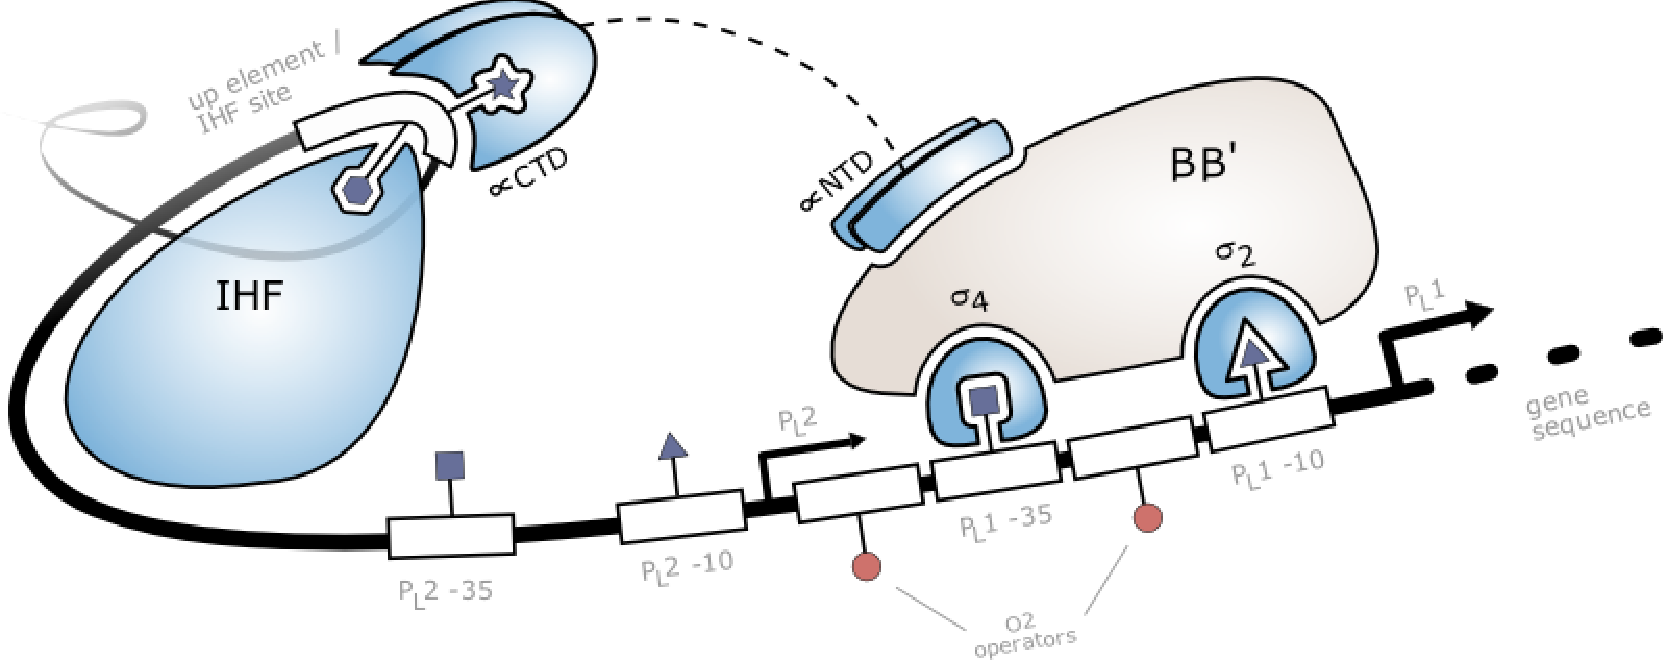
\includegraphics[width=6in]{Body/Images-chap4/fig1.pdf}

        \caption[Structure of the PL--TET01 promoter]{
            Structure of the PL--TET01 promoter.  There are a numerous functional sites on the  PL--TET01 promoter that are known to effect the rate of complex formation between the promoter and RNA polymerase~\cite{giladi1995enhanced,giladi1998participation,giladi1996identification}.  The promoter region contains two tandem promoters  PL--1 and  PL--2, each of which contain -10 and -35 sigma factor binding sites.  Furthermore, the promoter contains, at approximately the same location, an UP element that binds C--terminal domain of the alpha subunit and a binding site for integration host factor (IHF) a global regulator of gene expression in \emph{E. coli}.  The IHF site acts to bend the promoter region, brining the alpha--CTD binding site in sufficient proximity to the beta subunit of the RNA polymerase.  In addition, the  PL--TET01 promoter has two tetO2 operators from the Tn10 tetracycline resistance operon~\cite{lutz1997independent}.
        }
        \label{fig:pltet}
        \end{sidewaysfigure}


    Mutants in the library were analyzed using
    flow--cytometry to measure the single--cell level of
    expression of GFP  as a proxy for the activity of
    the mutagenized promoters.  (A detailed schematic of
    the experimental procedure is shown in Figure~\vref{fig:flowcyto}.)
    Promoters that had roughly log--normal fluorescence
    distributions (no obvious tails in the distribution
    or bimodal distributions) were sequenced and, from
    that set, those mutants that contained deletions or
    insertions were removed.  The final set comprised
    69 mutant promoters, with well--behaved fluorescence
    distributions (single distribution with a low standard
    deviation) , that only contained transition and
    transversion mutations.  Notably, our error--prone PCR
    method introduces predominantly transitions and not
    transversions, except in rare cases.

        \begin{figure}[phtb]
        \centering
        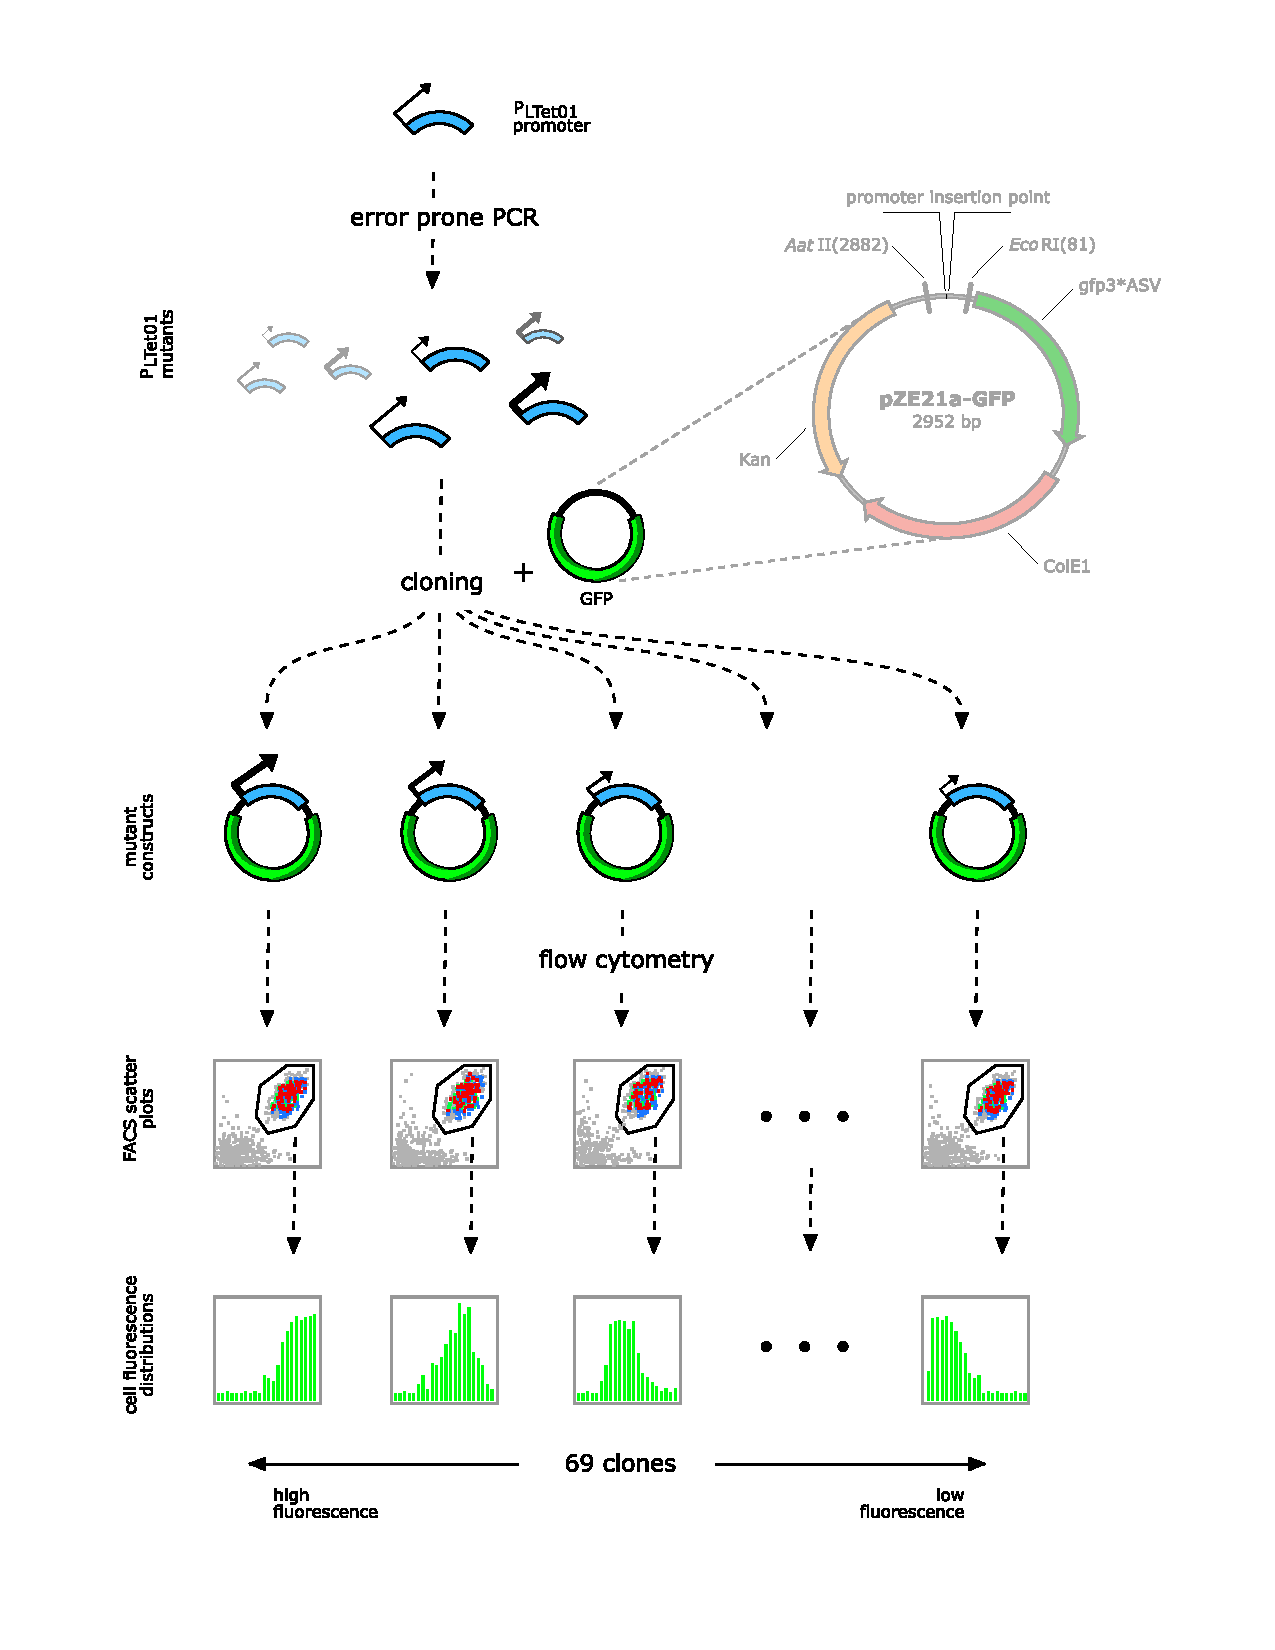
\includegraphics[width=\textwidth]{Body/Images-chap4/flowcyto.pdf}

        \caption[Schematic of the experimental procedure for promoter mutagenesis]{
            Schematic of the experimental procedure.  A variant of the constitutive bacteriophage PL--$\lambda$ promoter (PL--TETO1) was mutated through error--prone PCR to create mutated fragments of promoters.  These fragments were then ligated into plasmid constructs and used to drive the expression of \emph{gfp} in \emph{E.coli}.  These cells were then analyzed using flow cytometry to quantify the fluorescence of GFP and output capacity of the promoter.   }
        \label{fig:flowcyto}
        \end{figure}



\subsubsection{Identification of critical sites}

    Returning to the red, blue, green example
    introduced earlier, each of these N hypothetical
    mutants can be classified into one of M
    mutually--exclusive and collectively--exhaustive
    phenotypic classes --- $P_1, P_2,\ldots,P_M$ --- such
    that there are $n_1, n_2,\ldots,n_M$, mutants in each
    class and $\sum n_i=N$.  Consider a subset of mutants
    $B$ of size $X$, where $X<N$, comprising mutants with
    a particular mutation.  If the mutation does not
    influence the phenotype of the mutants, we would
    expect, by chance, that there would be $x_i=X(n_i/N)$
    mutants of type $P_i$.  In general, the probability
    that the set  ${x_1, x_2,\ldots,x_M}$ will take on the
    particular set of values ${y_1, y_2,\ldots,y_M}$ is
    \begin{equation}\label{eqn:pro-eq1}
        \pr{x_1=y_1,x_2=y_2,\dots,x_M=y_M}=\binom{X}{y_1,y_2,\ldots,y_M}\prod_{i=1}^{M}\frac{n_i}{N}
    \end{equation}
where $\sum y_i=X$.  In this equation, the term
    \begin{equation}\label{eqn:pro-eq2}
        \pr{x_1=y_1,x_2=y_2,\dots,x_M=y_M}=\binom{X}{y_1,y_2,\ldots,y_M}\prod_{i=1}^{M}\frac{n_i}{N}
    \end{equation}
is the so--called multinomial coefficient, which can be
equivalently written
    \begin{equation}\label{eqn:pro-eq3}
        \binom{X}{y_1,y_2,\ldots,y_M}=\frac{X!}{y_1!,y_2!,\ldots,y_M!}.
    \end{equation}


The coefficient is the number of ways sets of size
${y_1, y_2,...,y_M}$ could be chosen from a set of size X.
(For example, in the case $X=6, M=2, y_1=y_2=3$, the
coefficient is 20 because there are 20 different ways to
choose two subsets of size three from a set of six.)

    The probability that $q$ or more (where $q<X$) of the
    $B$ mutants would be seen in a particular class,
    $P_i$, by chance is
    \begin{equation}\label{eqn:pro-eq4}
        \pr{x_i\geq q} = \sum_{k=q}^{X}\binom{X}{q}\paren{\frac{n_i}{N}}^k\paren{1-\frac{n_i}{N}}^{N-k}.
    \end{equation}




Equivalently, this is the p--value for seeing $q$ of the $B$
mutants in class  $P_i$.  The lower the p--value, the more
confident we are that the $B$ mutation is correlated with
the $P_i$ phenotype.

    For this study, we divided the mutants into two
    phenotypic classes based on their fluorescence
    (i.e. $M=2$): the top 50th percentile and the
    lower 50th percentile.  Figure~\vref{fig:mutstats} shows a detailed
    schematic of the statistical analysis, which is
    greatly simplified in this case because there
    are only two phenotypes.  As shown in the figure,
    applying our statistical method to the sequence
    data resulted in the identification of seven
    nucleotide positions that are correlated with one
    of the two phenotypic classes in a statistically
    significant manner.  The figure should be read
    clockwise from the top--left, progressively
    showing the fluorescence distribution, mutation
    distribution, statistical distribution of
    mutations, and finally, the identified important
    positions in part D in the lower left.
    In quadrant A,
    the vertical axis shows the mutant number, where
    the mutants are sorted in descending order by their
    relative fluorescence.  In general, the single-cell
    fluorescence distribution for each mutant strain
    was log-normal distributed.  The horizontal axis
    shows the mean of the log relative fluorescence for
    each mutant strain, where the error is the standard
    deviation of this distribution.  Reading to the
    right from quadrant A into quadrant B reveals the
    point mutations present in each mutant.  For each
    location in a mutant (where location is indicated
    on the horizontal axis) that was changed via the
    error-prone PCR, a black dot is indicated.  With
    only a handful of exceptions, all of these changes
    are base transitions rather than transversions,
    so the sequence of each of the 69 clones can be
    inferred from the WT sequence shown in quadrant D.
    Reading down from quadrant B into quadrant C
    shows how mutations at a particular location
    partition between the two classes of mutants:
    the top and bottom 50th percentiles.  Sites that
    have no effect on the fluorescence phenotype should
    partition equally between the two classes, i.e.\ they
    should follow a binomial distribution with $p=0.5$.
    Sites that deviate from this distribution are
    labeled with a dot and are colored either green
    or red, corresponding to the apparent effect of a
    mutation at the site.  For these sites, p--values
    are indicated, where this value is the probability
    of seeing a distribution at least as skewed to
    one side.  Sites that were subsequently tested
    experimentally (see below) are indicated with an
    asterisk, where the color of the asterisk denotes
    the expected effect of a mutation at the site.
    We chose a range of sites to test experimentally,
    from those with high-confidence (low p--value)
    positive effects, to those with low-confidence
    (p--value $\sim$ 0.5) negative effects (see Table~\vref{table:sites1}).
    These sites are also shown in quadrant D, which
    contains the WT nucleotide sequence of the promoter
    region that was subjected to mutation.


        \begin{figure}[phtb]
        \centering
        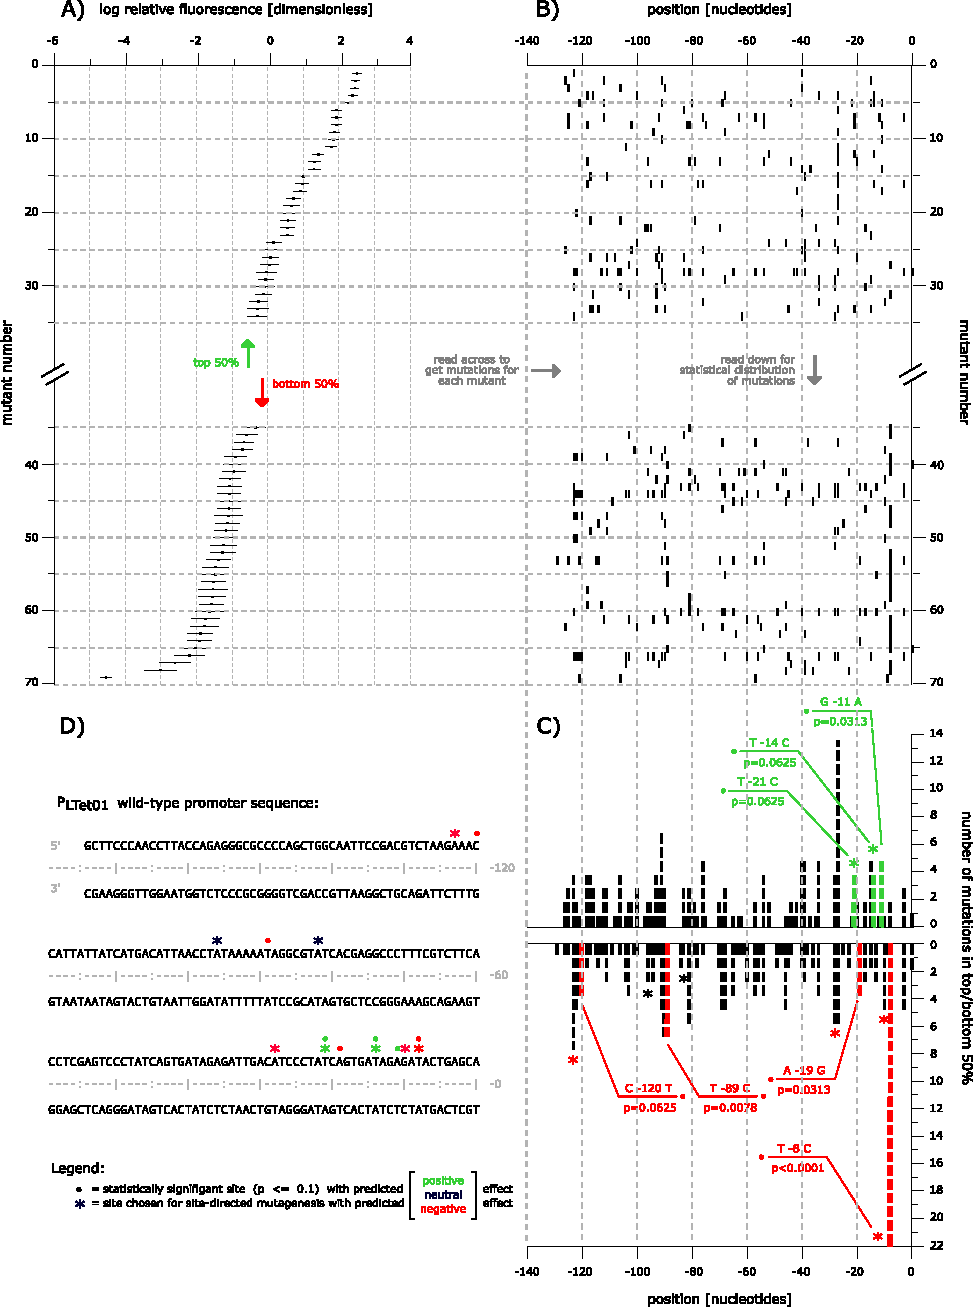
\includegraphics[width=\textwidth]{Body/Images-chap4/mutstats.pdf}
        \caption[Statistical distribution of mutations and their effects on mutant fluorescence]{
        Statistical distribution of mutations and their effects on mutant fluorescence.  See text for a description.
        }
        \label{fig:mutstats}
        \end{figure}


\subsubsection{Site--directed mutagenesis of predicted sites}

We selected 8 sites in the promoter region to test
whether their phenotypic effects, as predicted by the
statistical method, agreed with their observed effects when
the mutations were introduced individually, without the
background of other mutations.  These 8 mutated positions
are shown in Table~\vref{table:sites1} and labeled in Figure~\vref{fig:mutstats}, parts C\&D.  The sites
were chosen to span a range of characteristics.  The -8
site was predicted to have a negative effect on promoter
strength with high confidence, i.e. it was statistically
significant (see Table~\ref{table:sites1}).  The -10, -28, and -123 sites
were predicted to have negative effects, but had moderate
p--values and, thus, medium--to--low confidence.  Sites -14
and -21 were predicted to have positive effects with high
confidence.  The sites -82 and -96 were chosen because
they had p--values of exactly 0.5.  Notably, there are two
ways that a position could have produced an insignificant
p--value (i.e. a p--value close to 0.5): the mutation could
partition equally between the two classes, or the mutation
could have been observed very few times.  Mutations at both
the -82 and -96 sites were observed relatively few times
and seemed to partition between the top--50th percentile and
bottom--50th percentile classes with equal frequency.  Thus,
in the absence of a statistically significant correlation,
we predicted they would have no effect on the phenotype.
(These observations are summarized in Table~\vref{table:sites1}.)

    For each of the sites listed in Table~\vref{table:sites1}, we created
    mutant strains incorporating transition SNPs at
    the specified location.  Each of these mutants
    were analyzed using flow-cytometry to test the
    single-cell level of expression of GFP using the
    same protocols as for the parent mutant library.
    The fluorescence results for each mutant are shown
    in Table~\vref{table:sites1} in the right-most columns.  In addition,
    for certain combinations of sites in Table~\vref{table:sites1},
    we created double and triple mutants (see Table~\vref{table:sites2}).

\subsection{Discussion}

As shown in Table~\vref{table:sites1}, the statistical method correctly
predicts the phenotypic effects of 7/8 of the individual
mutations that were tested.  Furthermore, the phenotypic
effects of the mutations with statistically significant
p--values were correctly predicted. For these mutations,
we showed that the effect of an individual mutation on the
phenotype can be parsed out from a mutational spectrum,
even when the effect is obscured by a background of other
mutations.

It is interesting to note that while most of the
statistically significant mutations are near the sigma
factor binding sites, two are located further upstream of
this region.    The -123 site, which was not statistically
significant, but was tested experimentally, showed that
such distal sites are participating in the regulation
of transcription.

    There are a few caveats to the use of our
    statistical method.  First, the method assumes
    independence between mutations.  That is, we
    assume mutated sites cannot interact.  As shown in
    Table~\vref{table:sites2}, 4/6 of the combination--mutations had the
    predicted effect.  The two combination--mutants
    that had unintuitive phenotypes could be a
    result of interaction between sites.  (Notably,
    the -82,-14,-21 triple mutant appeared to have a
    high fluorescence by visual inspection in a rich
    medium pre--culture; however, quantification of GFP
    activity by flow cytometry revealed consistently
    low measurements in the minimal medium used.)

    The second caveat is that the method can require
    a significant number of mutants for each position:
    for a position to be statistically significant in
    our particular experiment, at least 4 observations
    were required.  (This would be true for any
    two--phenotype mutational spectra, where each
    phenotype occurs with equal prior probability.)
    The number of observations required scales
    roughly with the number of mutation types. Our
    mutagenesis method introduced only transitions,
    not transversions, which allowed us to treat each
    site as "mutated" or "not mutated" without loss
    of information.  The method can by applied to
    cases in which all four nucleotides are present;
    however, roughly 4 times as many observations would
    be required to make a statistically significant
    correlation between a particular nucleotide (at
    a single position) and a phenotype.  Finally,
    the statistical method presented here is only
    applicable to situations in which the method
    used to introduce sequence diversity does not
    also introduce deletions or insertions.  Ignoring
    relatively small insertions or deletions in the
    analysis would not significantly bias the results
    of identifying critical residues (data not shown).
    However, rigorously, alterations would be needed
    to differentiate between deletions and mutations
    in our statistical framework.  In such cases,
    more complex models could be adapted, such as
    those used to describe the distribution and
    effects of  naturally--occurring mutations over a
    fitness landscape for populations under positive
    and negative selective pressures~\cite{orr2003minimum,rokyta2005empirical}.

Despite its caveats, this method has a significant
advantage when compared to deducing critical mutations
using sequence data from only the best performing mutants.
Intuitively, if we were to ignore the bottom--50th
percentile in Figure~\ref{fig:mutstats} part C on page~\pageref{fig:mutstats}, we may mistakenly identify sites
as associated with high fluorescence that are, in fact,
evenly distributed between the two classes.  That is,
having sequence data for multiple phenotypes allowed us
to determine, with quantifiable confidence, the effect of
each individual mutation in a way that discounts artifacts
of the mutagenesis method, such as a bias for mutagenizing
particular loci.








    \begin{sidewaystable}[ptb]
    \caption[Summary of site--directed mutagenesis loci]{Summary of site--directed mutagenesis loci.  The selected sites, which span a range of p--values and predicted activities, were each mutated and assayed for fluorescence levels individually (see Figure~\vref{fig:mutstats}.  As shown in the table, all sites but the -96 site were in the phenotypic class predicted by our statistical method.
        }\label{table:sites1}
    \centering
    \begin{tabular}{cccccccc} \hline \hline
Site
&
Predicted activity
&
P--value
&
Observations
&
Confidence
&
Relative Fluorescence
&
Log Relative Fluorescence
&
Agreement?
\\
-8
&
Low
&
<0.0001
&
22
&
High
&
0.036
&
-3.32
&
Yes
\\
-10
&
Low
&
0.1094
&
6
&
Med
&
0.011
&
-4.52
&
Yes
\\
-14
&
High
&
0.0625
&
4
&
High
&
1.428
&
0.35
&
Yes
\\
-21
&
High
&
0.0625
&
4
&
High
&
1.585
&
0.46
&
Yes
\\
-28
&
Low
&
0.3770
&
10
&
Low
&
0.756
&
-2.58
&
Yes
\\
-82
&
No effect
&
0.5000
&
2
&
Low
&
0.926
&
-0.08
&
Yes
\\
-96
&
No effect
&
0.5000
&
5
&
Med
&
0.046
&
-3.08
&
No
\\
-123
&
Low
&
0.1938
&
12
&
Med
&
0.087
&
-2.45
&
Yes \\ \hline \hline
    \end{tabular}
    \end{sidewaystable}





    \begin{sidewaystable}[ptb]
    \caption{Summary of double and triple mutants constructed by site--directed mutagenesis.}\label{table:sites2}
    \centering
    \begin{tabular}{ccccc} \hline \hline
Sites
&
Predicted activity
&
Relative Fluorescence
&
Log Relative Fluorescence
&
Agreement?
\\
-14, -21
&
High
&
1.924
&
0.65
&
Yes
\\
-14, -82
&
High
&
0.954
&
-0.04
&
No
\\
-21, -82
&
High
&
1.433
&
0.36
&
Yes
\\
-96, -123
&
Low
&
0.274
&
-1.43
&
Yes
\\
-82,-14,-21
&
High
&
0.140
&
-1.97
&
No
\\
-8,-10,-28
&
Low
&
0.018
&
-4.03
&
Yes
\\
\hline \hline
    \end{tabular}
    \end{sidewaystable}
